\documentclass[a4paper, 11pt]{article}
\usepackage[letterpaper,margin=0.8in]{geometry}
\usepackage{blindtext}
\usepackage{lastpage}
\usepackage{fancyhdr}
\usepackage{xcolor}
\usepackage{setspace}
\usepackage{amsmath}
\usepackage{graphicx}
\usepackage{matlab-prettifier}
\usepackage{float}
\usepackage{multirow}
\definecolor{codemagenta}{rgb}{1,0,0.5}
\definecolor{codegray}{rgb}{0.4,0.4,0.4}
\definecolor{codepurple}{rgb}{0.8,0.2,1}
\definecolor{codeorange}{rgb}{1,0.6,0}
\definecolor{codecyan}{rgb}{0,0.8,1}
\definecolor{codebrown}{rgb}{0.7,0.5,0.3}
\definecolor{codered}{rgb}{1,0.2,0.2}
\definecolor{backcolour}{rgb}{1,1,1}
\lstset{
    language=Python,
    backgroundcolor=\color{backcolour},
    commentstyle=\color{codegray}\itshape,
    keywordstyle=\color{codepurple}\bfseries,
    numberstyle=\tiny\color{codebrown},
    stringstyle=\color{codemagenta}\bfseries,
    basicstyle=\ttfamily\small\color{black},
    emph={True,False,None,self,def,class,return,import,from,as,if,else,elif,for,while,in},
    emphstyle=\color{codepurple}\bfseries,
    emph={[2]np,plt,import,from},
    emphstyle={[2]\color{codeorange}\bfseries},
    breakatwhitespace=false,
    breaklines=true,
    captionpos=b,
    keepspaces=true,
    showspaces=false,
    showstringspaces=false,
    showtabs=false,
    tabsize=4,
    morekeywords={True,False,None}
}
\usepackage[small,bf,hypcap=true]{caption}

\newenvironment{Figure}
  {\par\medskip\noindent\minipage{\linewidth}
   \captionsetup{type=figure}}
  {\endminipage\par\medskip}
\usepackage[hidelinks]{hyperref}
\usepackage{titlesec}
\usepackage{tocloft}

\renewcommand{\cftsecleader}{\cftdotfill{\cftdotsep}}

\graphicspath{{./Figures}}

% Configure the header
\pagestyle{fancy}
\fancyhead[L]{CE 598}
\fancyhead[C]{Coastal \& Harbour Structures Design}
\fancyhead[R]{25/02/2026}

\setlength{\floatsep}{6pt plus 2pt minus 2pt}
\setlength{\textfloatsep}{8pt plus 2pt minus 2pt}
\setlength{\intextsep}{8pt plus 2pt minus 2pt}

\onehalfspacing

\begin{document}

\titleformat{\section}
  {\normalfont\bfseries\fontsize{12}{10}\selectfont}
  {\large\thesection.} 
  {0.3em}
  {}

\thispagestyle{empty}
% -------------------- Title Page --------------------
\begin{titlepage}
    \begin{figure}[H]
        \vspace{0.6cm}
        \centering
        
\includegraphics[width=0.45\textwidth]{logo.png}
    \end{figure}
    \vspace{0.8cm}

    \centering
    \textbf{\LARGE Middle East Technical University}\\[0.3cm]

    \textbf{\LARGE Department of Civil Engineering}\\[0.5cm]

    \textbf{\Large 2025-2026 Spring Semester}\\[1.5cm]

    \textbf{\Large CE598 Coastal \& Harbour Structures Design}\\[0.9cm]

    \textbf{\LARGE Term Project - Part 1 }\\[1.5cm]

    \large Instructor:

    \large Dr. Işıkhan Güler\\[1.2cm]

    \large Submitted by:
    
    \large Bilge Kutay
    
    \large 2511798\\[1.5cm]

\end{titlepage}

% -------------------- Table of Contents --------------------
\newpage
\renewcommand{\contentsname}{Table of Contents} 
\begin{center}
    \tableofcontents
\end{center}
\newpage

\listoffigures
\listoftables
\newpage


% -------------------- Introduction --------------------
\section{Introduction}

\hspace*{0.5cm}This study examines the wind-wave climate in the Tekirdağ region of the Sea of Marmara using ERA5 wind data at the grid point 
40.75°N, 27.75°E, selected offshore of Tekirdağ Limanı. The analysis covers the period 1985-2024 and is based on hourly wind records. Because the study area is located in a semi-enclosed basin, wave development is mainly controlled by local wind conditions and the limited directional fetch available at the site.

The aim of the study is to estimate the wave heights and peak periods that can develop at this location under local wind forcing. For this purpose, effective fetch lengths were determined for the selected point, the wind record was separated into individual storm events, and the corresponding significant wave heights and peak periods were hindcast using the JONSWAP method. The resulting wave series was then analyzed to determine both frequently occurring severe conditions and rare extreme conditions relevant to coastal engineering applications.

The study focuses on two main outputs. The first is the significant wave height exceeded for 10 hours per year, obtained from the long-term wave statistics of the hourly hindcast series. The second is the 100-year return period significant wave height, estimated from annual maximum wave heights obtained from the storm-based analysis. In this way, the study provides a site-specific assessment of the wave climate in the Tekirdağ coastal area based on long-term wind forcing and fetch-limited wave growth in the Sea of Marmara.

% -------------------- Methodology --------------------
\section{Methodology}

\subsection{Wind Data and Study Point}

\hspace*{0.5cm}Hourly wind data were extracted from ERA5 reanalysis NetCDF files at the grid point 40.75°N, 27.75°E. The 10-metre wind components, $u_{10}$ and $v_{10}$, were used to compute the wind speed and meteorological wind direction at each hour:

\begin{equation}
    U = \sqrt{u_{10}^2 + v_{10}^2}
\end{equation}

Wind direction was also calculated for each hour and used later to assign fetch values from the directional fetch table. These wind speed and direction data were then used in the storm analysis and wave calculations.

\begin{equation}
    \theta = \mod\left(\mathrm{atan2}(-u_{10},\, -v_{10}) \cdot \frac{180}{\pi},\; 360\right)
\end{equation}

\subsection{Effective Fetch Calculation}

\hspace*{0.5cm}Fetch values for the study point were calculated separately before the main wave analysis. Since the study area is located in the Sea of Marmara, the available fetch changes a lot with direction, so a single fetch value is not enough to represent the site. For this reason, effective fetch lengths were calculated for 16 main directions at \(22.5^\circ\) intervals.

The Shore Protection Manual effective fetch approach was used with the \(\pm42^\circ\) method. For each main direction, additional rays were taken within a \(\pm42^\circ\) range, and the distances along these rays were combined using cosine weighting. In this way, one effective fetch value was obtained for each of the 16 directions.

The coastline geometry used in the fetch calculation was taken from the GSHHG shoreline dataset. After the coastline data were clipped to the Sea of Marmara region, the study point and coastline were projected into a metric coordinate system so that fetch lengths could be measured in meters. The final fetch values were then stored as a directional fetch table.

During the wave analysis, the fetch corresponding to each hourly wind direction was obtained by interpolating between these directional fetch values. This made it possible to assign a fetch length to every hourly wind record used in the storm and wave calculations.

\begin{figure}[H]
    \centering
    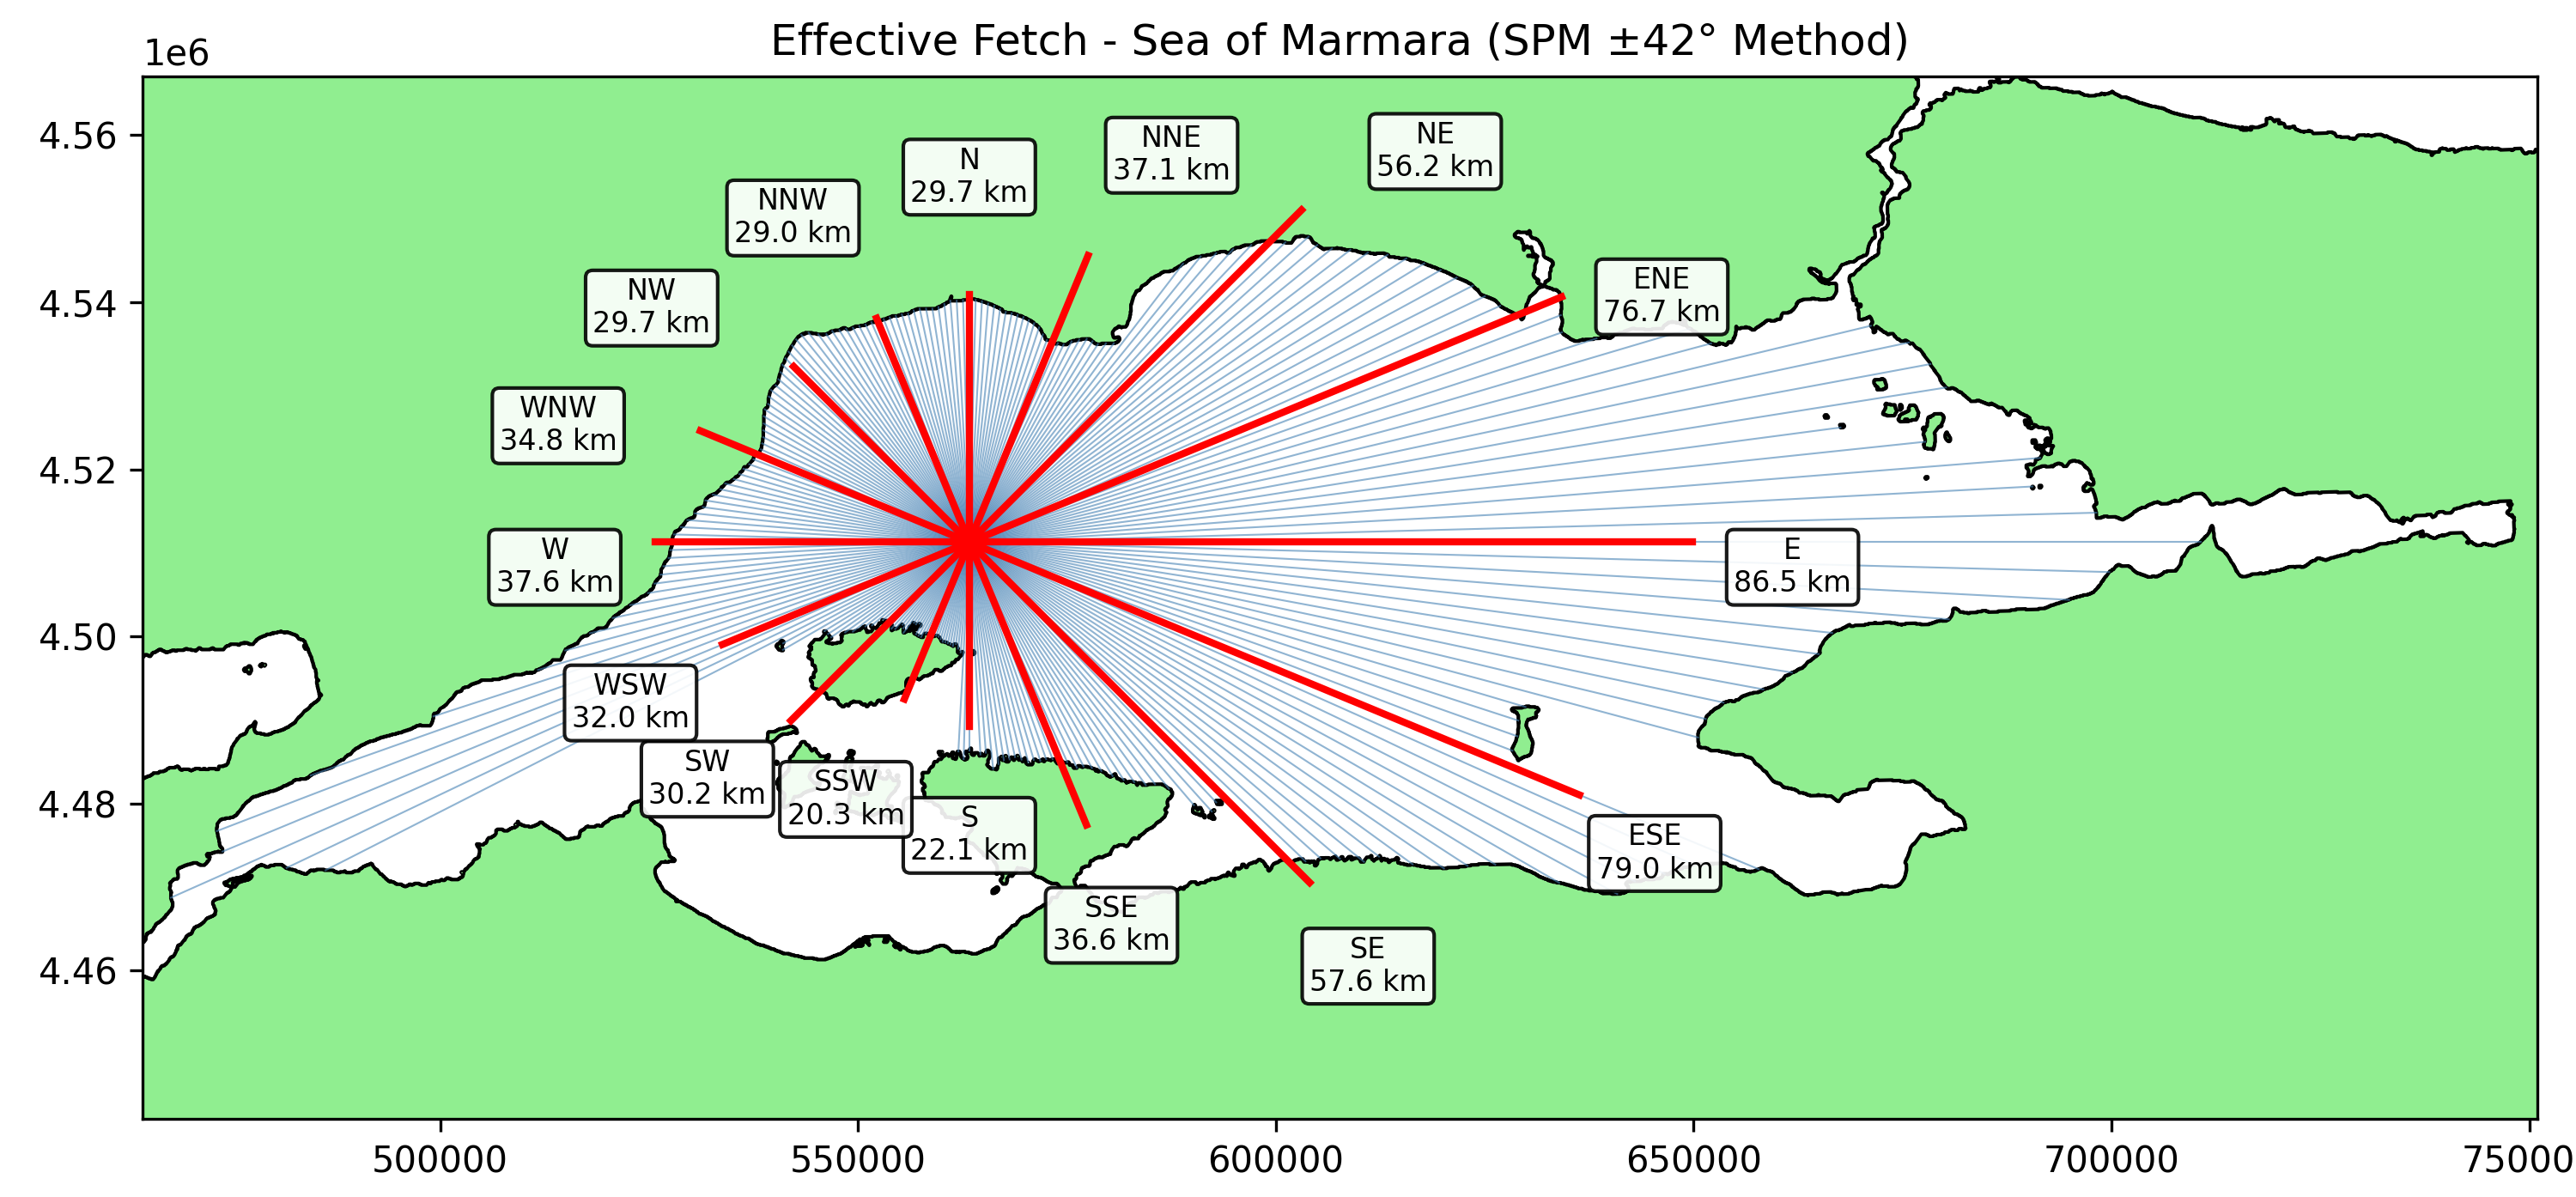
\includegraphics[width=0.85\textwidth]{effective_fetch_map.png}
    \caption{Effective fetch map for the study point offshore of Tekirdağ Limanı.}
    \label{fig:fetch_map}
\end{figure}

\subsection{Storm identification}

\hspace*{0.5cm}After the wind data were processed, the full time series was divided into individual storm events. In this study, a storm was defined as a continuous period during which the wind speed remained equal to or greater than \(3\ \mathrm{m/s}\). Once the wind speed dropped below this value, the storm was considered to have ended, and a new storm began only when the threshold was exceeded again.

For each storm, the duration was taken as the total number of consecutive storm hours. The representative wind speed of the storm was taken as the average wind speed over the whole storm. In addition, the fetch values corresponding to the hourly wind directions within the same storm were checked, and the direction associated with the maximum fetch was selected as the representative storm direction. The fetch value in that direction was then used in the wave calculations.

Using this procedure, each storm was represented by three main parameters; a representative wind speed, fetch, and a storm duration. These values were then used in the hindcasting step.

\subsection{Wave Hindcasting using JONSWAP}

\hspace*{0.5cm}The JONSWAP method was used to estimate the significant wave height \(H_s\) and peak period \(T_p\) for each storm based on the representative wind speed and fetch. In the calculations, the wind stress factor was first obtained from the representative wind speed as

\[
U_A = 0.71\,U^{1.23}
\]

where \(U\) is the representative storm wind speed. Using \(U_A\), the dimensionless fetch and dimensionless duration were calculated as

\[
F^*=\frac{gF}{U_A^2}
\qquad
t^*=\frac{gt}{U_A}
\]

where \(F\) is the fetch length, \(t\) is the storm duration, and \(g\) is the gravitational acceleration.

The fully developed sea limits were taken as

\[
H_s^* = 0.243
\qquad
T_p^* = 8.13
\]

and their dimensional forms were written as

\[
H_{s,\mathrm{FD}} = 0.243\,\frac{U_A^2}{g}
\qquad
T_{p,\mathrm{FD}} = 8.13\,\frac{U_A}{g}
\]

The effective dimensionless fetch based on duration was calculated from

\[
F^*_{\mathrm{eff}}=\left(\frac{t^*}{68.8}\right)^{3/2}
\]

The controlling fetch term in the calculation was taken as the smaller of \(F^*\) and \(F^*_{\mathrm{eff}}\). Using this value, the developing sea relations were written as

\[
H_s^* = 0.0016\left(F^*_{\mathrm{eff}}\right)^{1/2}
\qquad
T_p^* = 0.286\left(F^*_{\mathrm{eff}}\right)^{1/3}
\]

Their dimensional forms were then obtained as

\[
H_{s,\mathrm{D}} = H_s^*\,\frac{U_A^2}{g}
\qquad
T_{p,\mathrm{D}} = T_p^*\,\frac{U_A}{g}
\]

Finally, the significant wave height and peak period for each storm were taken as the smaller of the fully developed and developing-sea values:

\[
H_s = \min\left(H_{s,\mathrm{FD}},\,H_{s,\mathrm{D}}\right)
\qquad
T_p = \min\left(T_{p,\mathrm{FD}},\,T_{p,\mathrm{D}}\right)
\]

In this way, one significant wave height and one peak period were obtained for each storm.

In addition to the storm-based calculations, hourly wave heights were also estimated within each storm by using the hourly wind speed, hourly fetch, and elapsed storm duration. These hourly values were later used in the long-term wave statistics analysis.

\subsection{Extreme Wave Analysis}
\hspace*{0.5cm}Extreme wave analysis was carried out using the annual maxima series obtained from the storm-based wave calculations. For each year in the record, the largest significant wave height was selected together with its corresponding peak period and direction. This annual maxima series was then used to fit several candidate probability distributions and estimate the 100-year return period wave height.

\subsubsection{Distributions and Fitting Procedure}
In this study, ten candidate distributions were tested in the extreme value analysis. These were the old Gumbel distribution, the new Gumbel distribution, Fr\'echet Type II distributions with \(k=2.5\), \(3.33\), \(5.0\), and \(10.0\), and Weibull distributions with \(k=0.75\), \(1.0\), \(1.4\), and \(2.0\).

For each candidate distribution, the required plotting-position constants and shape parameters were taken from the reference tables provided in the course material. These tables were used directly in the code for defining the distribution parameters and for carrying out the fitting procedure. The reference tables used for the candidate distributions are given in \autoref{tab:dist_constants_table}.
\vspace{0.2cm}

\begin{table}[H]
    \centering
    \caption{Reference table used for the extreme value distributions, including plotting-position constants and shape parameters.}
    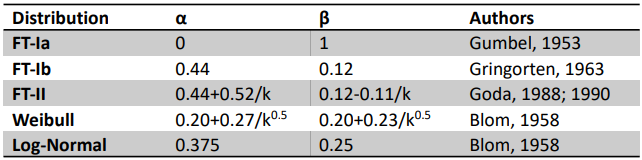
\includegraphics[width=0.7\textwidth]{distribution_constants_table.png}
    \label{tab:dist_constants_table}
\end{table}

For all candidate distributions, the annual maxima series was first ranked in descending order. The plotting position for each ranked value was then calculated as
\[
F_i = 1-\frac{i-a}{n+b}
\]

where \(i\) is the rank, \(n\) is the number of annual maxima, and \(a\) and \(b\) are the plotting-position constants corresponding to the selected distribution.

For the old and new Gumbel distributions, the reduced variate was written as
\[
y = -\ln\left[-\ln(F_i)\right]
\]

For the Fr\'echet Type II distributions, the reduced variate was written as
\[
y = \left[-\ln(F_i)\right]^{-1/k}-1
\]
where \(k\) is the shape parameter.

For the Weibull distributions, the reduced variate was written as
\[
y = \left[-\ln(1-F_i)\right]^{1/k}
\]

After the reduced variates were obtained, a linear relation of the form
\[
x = Ay + B
\]
was fitted to the annual maximum significant wave heights, where \(x\) represents the annual maximum wave height and \(A\) and \(B\) are the fitting constants. These constants were obtained from the variance and covariance of the transformed data and wave height values. Once \(A\) and \(B\) were determined, each candidate distribution could be used to estimate return period wave heights, including the 100-year significant wave height.

\subsubsection{Goodness-of-fit Tests and Distribution Selection}

\hspace{0.5cm}After fitting each candidate distribution, several goodness-of-fit tests were used to compare their performance. In this study, the coefficient of determination \(R^2\), the mean integrated residual (MIR) test, the REC test, the DOL test, and the Kolmogorov--Smirnov (KS) test were applied.

\paragraph{Coefficient of determination \texorpdfstring{$R^2$}{R2}:}
The coefficient of determination \(R^2\) was used to evaluate how well the fitted straight line represented the transformed annual maxima data in reduced-variate space. In the calculations, the correlation coefficient was first written as

\[
r = \frac{\mathrm{Cov}(Y,X)}{\sqrt{\mathrm{Var}(X)\mathrm{Var}(Y)}}
\qquad
R^2 = r^2
\]

Higher \(R^2\) values indicate a better fit between the transformed data and the fitted line.

\paragraph{Mean integrated residual (MIR):}
For the MIR test, the residual quantity was first defined as

\[
\Delta_r = 1-r
\]

This value was then compared with the reference mean residual value \(\Delta_{r,\mathrm{mean}}\), which was calculated from the number of data points \(n\) in the annual maxima series using the empirical relation:

\[
\Delta_{r,\mathrm{mean}}=
\exp\left(a + b\ln(n) + c[\ln(n)]^2\right)
\]

where \(a\), \(b\), and \(c\) are the empirical constants given in \autoref{tab:MIR_coeff}.

\begin{table}[H]
    \centering
    \caption{Empirical constants used in the MIR test.}
    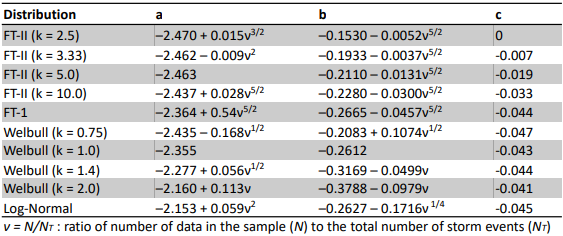
\includegraphics[width=0.7\textwidth]{MIR_coeff.png}
    \label{tab:MIR_coeff}
\end{table}

The MIR statistic was then calculated as

\[
\mathrm{MIR} = \frac{\Delta_r}{\Delta_{r,\mathrm{mean}}}
\]

Lower MIR values indicate better agreement between the fitted distribution and the annual maxima data.

\paragraph{Deviation of Outlier (DOL) Criterion:}
For the DOL test, the purpose was to check whether the largest annual maximum behaved as an outlier relative to the rest of the sample. In the code, the test statistic was calculated as

\[
\xi = \frac{x_1-\bar{x}}{s^2}
\]

where \(x_1\) is the largest annual maximum, \(\bar{x}\) is the sample mean, and \(s^2\) is the standard deviation. This value was then compared with the upper and lower critical values corresponding to the 95\% confidence level, which were calculated from the number of data points \(n\) in the annual maxima series using the relations:

\[
\xi_{95} = a_{95} + b_{95}\ln(n) + c_{95}[\ln(n)]^2
\]

\[
\xi_{5} = a_{5} + b_{5}\ln(n) + c_{5}[\ln(n)]^2
\]

where \(a_{95}\), \(b_{95}\), \(c_{95}\), \(a_{5}\), \(b_{5}\), and \(c_{5}\) are the empirical constants given in \autoref{tab:DOL_coeff} and \autoref{tab:DOL_coeff2}.

\begin{table}[H]
    \centering
    \caption{Empirical constants used in the DOL test for the 95\% confidence level.}
    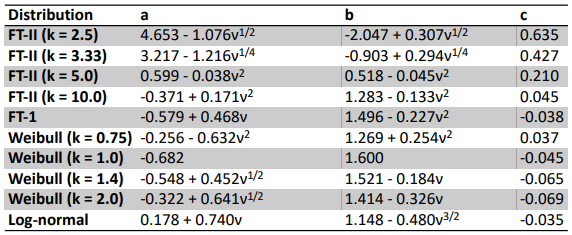
\includegraphics[width=0.7\textwidth]{DOL_coeff_95.png}
    \label{tab:DOL_coeff}
\end{table}

\begin{table}[H]
    \centering
    \caption{Empirical constants used in the DOL test for the 5\% confidence level.}
    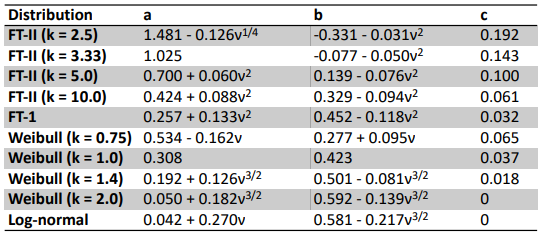
\includegraphics[width=0.7\textwidth]{DOL_coeff_5.png}
    \label{tab:DOL_coeff2}
\end{table}

If the calculated value satisfied

\[
\xi_5 < \xi < \xi_{95}
\]

the distribution was accepted in terms of the DOL test.

\paragraph{Residue of Correlation Coefficient (REC) Criterion:}
For the REC test, the residual \(\Delta_r\) was compared with the critical limit \(\Delta_{r,95}\), which was calculated from the number of data points \(n\) in the annual maxima series using the relation:

\[
\Delta_{r,95}=
\exp\left(a + b\ln(n) + c[\ln(n)]^2\right)
\]

where \(a\), \(b\), and \(c\) are the empirical constants given in \autoref{tab:REC_coeff}.

\begin{table}[H]
    \centering
    \caption{Empirical constants used in the REC test.}
    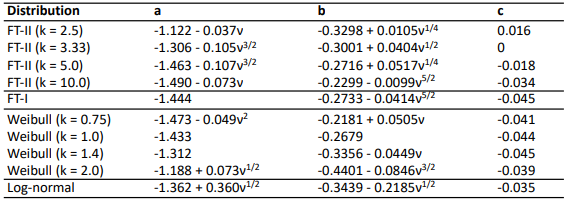
\includegraphics[width=0.7\textwidth]{REC_coeff.png}
    \label{tab:REC_coeff}
\end{table}

If the condition

\[
\Delta_r < \Delta_{r,95}
\]

was satisfied, the distribution was accepted in terms of the REC test.

\paragraph{Kolmogorov--Smirnov (KS) Test:}
For the Kolmogorov--Smirnov test, the empirical and theoretical cumulative distributions were compared. In the code, the empirical bounds were written as

\[
S_1=\frac{i-1}{n}
\qquad
S_2=\frac{i}{n}
\]

and the theoretical cumulative distribution values were obtained from the fitted distribution. Then the differences were calculated as

\[
D_1 = F(x)-S_1
\qquad
D_2 = S_2-F(x)
\]

and the KS test statistic was taken as

\[
D_{\mathrm{KS}} = \max\left(\max(D_1),\max(D_2)\right)
\]

In this study, the distribution was accepted if

\[
D_{\mathrm{KS}} < d_{\mathrm{crit}}
\]

where \(d_{\mathrm{crit}}=0.24\) was used in the code.
\vspace{0.5cm}

After all tests were completed, a scoring procedure was applied to compare the candidate distributions. The distributions were ranked according to their \(R^2\) and MIR values, while the REC, DOL, and KS tests were evaluated as accepted or not accepted. Scores were assigned to each criterion and summed to obtain a total score for each distribution. The distributions with the highest two scores were then selected for the final return period plots and the 100-year wave height estimation.

\subsubsection{Return Period Estimation}

After the candidate distributions were fitted and evaluated, the best-performing distributions were used to estimate return period wave heights. In this study, the return period analysis was based on the fitted linear relation

\[
x = Ay + B
\]

where \(x\) represents the significant wave height and \(y\) is the reduced variate corresponding to the selected distribution.

For a given return period \(T\), the non-exceedance probability was written as

\[
F = 1-\frac{1}{T}
\]

Using this probability, the reduced variate corresponding to the chosen distribution was calculated. For the Gumbel distributions, the reduced variate was written as

\[
y = -\ln\left[-\ln(F)\right]
\]

For the Fr\'echet Type II distributions, it was written as

\[
y = \left[-\ln(F)\right]^{-1/k}-1
\]

and for the Weibull distributions as

\[
y = \left[-\ln(1-F)\right]^{1/k}
\]

Once the reduced variate for the selected return period was obtained, the corresponding significant wave height was calculated from the fitted linear relation. In this way, return period wave heights could be estimated directly from the fitted distribution.

In the present study, the main design value obtained from this step was the 100-year return period significant wave height. After the 100-year wave height was determined, the corresponding peak period was estimated from the wave steepness relation used in the study. Return period plots were then prepared for the best-ranked distributions together with the fitted line and confidence bounds.


\subsection{Long Term Wave Statistics}
\hspace*{0.5cm}In addition to the extreme wave analysis, long-term wave statistics were obtained from the hourly significant wave height series calculated during the storm-based hindcasting step. For this purpose, the hourly wave heights were grouped into bins with a width of \(0.1\ \mathrm{m}\), and the cumulative exceedance frequency for each bin was calculated.

If \(H'\) denotes a given wave height level, the cumulative exceedance probability was written as

\[
Q(H_s > H') = \frac{N(H_s \geq H')}{N_{\mathrm{total}}}
\]

where \(N(H_s \geq H')\) is the number of hourly values greater than or equal to \(H'\), and \(N_{\mathrm{total}}\) is the total number of hourly records in the series.

After the exceedance probabilities were obtained, a logarithmic relationship was fitted between significant wave height and cumulative exceedance probability as

\[
H_s = A \ln(Q) + B
\]

where \(A\) and \(B\) are fitting constants obtained from the data. This fitted relation was then used to estimate wave heights corresponding to selected exceedance durations.

In this study, the main long-term wave statistic was the significant wave height exceeded for 10 hours per year. The corresponding exceedance probability was calculated as

\[
Q_{10} = \frac{10}{365.25 \times 24}
\]

and the associated significant wave height was obtained by substituting this value into the fitted relation. After the wave height for 10 hours per year was determined, the corresponding peak period was estimated using the wave steepness relation adopted in the analysis. The long-term wave statistics plot was then prepared by showing the cumulative exceedance data together with the fitted curve and the 10 hours per year point.

% -------------------- Results and Discussion --------------------
\section{Results and Discussion}

\hspace{0.5cm}The storm-based wave analysis showed that the wave climate at the selected offshore point near Tekirdağ is clearly controlled by directional exposure and fetch limitation. As seen earlier from the fetch calculation, the longest effective fetches occur mainly in the eastern and northeastern sectors. This pattern is reflected directly in the storm and annual maximum results. The largest wave conditions in the dataset were generally associated with storms coming from the \(E\), \(ENE\), and \(NE\) directions, while directions with shorter available fetch did not produce comparable wave heights even when wind speeds were relatively strong.

The annual maxima obtained from the storm-based wave series are listed in Table~\ref{tab:annual_maxima}. The results show that the yearly maximum significant wave heights remain within a relatively narrow range, from about \(1.517\ \mathrm{m}\) to \(2.186\ \mathrm{m}\). The largest annual maximum occurred in 2006, with \(H_s = 2.186\ \mathrm{m}\) and \(T_p = 6.709\ \mathrm{s}\). In general, the associated peak periods are also consistent, mostly falling between about \(5.8\ \mathrm{s}\) and \(6.7\ \mathrm{s}\). The directions of the annual maxima are concentrated mainly in the \(E\), \(ENE\), and \(NE\) sectors, which is fully consistent with the directional fetch pattern of the site.

\begin{table}[H]
    \centering
    \caption{Annual maximum significant wave heights, associated peak periods, and directions.}
    \label{tab:annual_maxima}
    \begin{tabular}{cccc}
\hline
Year & $H_s$ (m) & $T_p$ (s) & Direction \\
\hline
1985 & 1.703 & 6.200 & E \\
1986 & 1.670 & 6.160 & E \\
1987 & 1.925 & 6.331 & ENE \\
1988 & 1.776 & 6.163 & ENE \\
1989 & 1.633 & 5.690 & NE \\
1990 & 1.715 & 6.215 & E \\
1991 & 1.954 & 6.362 & ENE \\
1992 & 1.974 & 6.384 & ENE \\
1993 & 1.819 & 6.338 & E \\
1994 & 1.940 & 6.476 & E \\
1995 & 1.855 & 6.253 & ENE \\
1996 & 1.930 & 6.017 & NE \\
1997 & 1.809 & 6.327 & E \\
1998 & 1.699 & 6.195 & E \\
1999 & 1.741 & 6.122 & ENE \\
2000 & 1.668 & 6.035 & ENE \\
2001 & 2.053 & 6.598 & E \\
2002 & 1.876 & 6.276 & ENE \\
2003 & 1.791 & 6.180 & ENE \\
2004 & 1.947 & 6.355 & ENE \\
2005 & 1.784 & 6.297 & E \\
2006 & 2.215 & 6.768 & E \\
2007 & 1.880 & 6.281 & ENE \\
2008 & 1.820 & 6.339 & E \\
2009 & 1.544 & 6.001 & E \\
2010 & 1.765 & 6.274 & E \\
2011 & 2.006 & 6.418 & ENE \\
2012 & 1.673 & 6.163 & E \\
2013 & 1.579 & 6.045 & E \\
2014 & 1.658 & 5.742 & SE \\
2015 & 1.729 & 6.231 & E \\
2016 & 2.236 & 6.655 & ENE \\
2017 & 1.695 & 6.068 & ENE \\
2018 & 2.038 & 6.583 & E \\
2019 & 1.870 & 5.953 & NE \\
2020 & 2.046 & 6.461 & ENE \\
2021 & 1.701 & 6.075 & ENE \\
2022 & 1.797 & 6.187 & ENE \\
2023 & 1.890 & 6.292 & ENE \\
2024 & 1.982 & 6.393 & ENE \\
\hline
\end{tabular}

\end{table}

The top storm events provide a clearer view of the conditions producing the largest wave heights. The ten largest storm wave heights are given in Table~\ref{tab:top10_storms}. These results show that the largest events were not necessarily associated with the highest wind speed alone, but rather with the combination of sustained storm duration, relatively high wind speed, and favorable fetch direction. For example, the largest storm in 2016 produced \(H_s = 2.236\ \mathrm{m}\) with a peak fetch of \(76.716\ \mathrm{km}\), while other large storms in 2006, 2001, 2020, and 2018 were again associated with long fetches in the eastern and northeastern sectors. This confirms that the largest waves at the site develop when strong storms are aligned with the more exposed directions of the basin.

\begin{table}[H]
    \centering
    \caption{Top ten storm events ranked by significant wave height.}
    \label{tab:top10_storms}
    \begin{tabular}{ccccccc}
\hline
Year & Duration (hr) & $U_{max}$ (m/s) & Direction & Peak Fetch (km) & $H_s$ (m) & $T_p$ (s) \\
\hline
2016 & 65 & 17.208 & ENE & 76.716 & 2.236 & 6.655 \\
2006 & 144 & 17.858 & E & 86.517 & 2.215 & 6.768 \\
2001 & 113 & 16.351 & E & 86.517 & 2.053 & 6.598 \\
2020 & 117 & 18.116 & ENE & 76.716 & 2.046 & 6.461 \\
2018 & 32 & 14.217 & E & 86.517 & 2.038 & 6.583 \\
2001 & 394 & 17.035 & E & 86.517 & 2.015 & 6.558 \\
2006 & 100 & 15.603 & ENE & 76.716 & 2.014 & 6.427 \\
2011 & 96 & 15.885 & ENE & 76.716 & 2.006 & 6.418 \\
2024 & 70 & 15.082 & ENE & 76.716 & 1.982 & 6.393 \\
1992 & 221 & 16.106 & ENE & 76.716 & 1.974 & 6.384 \\
\hline
\end{tabular}

\end{table}

The annual maxima series was fitted using ten candidate distributions, and their performances were compared using the \(R^2\), MIR, REC, DOL, and KS criteria. The final ranking obtained from these tests is given in Table~\ref{tab:score_table}. According to the total score, the best-performing distribution was Gumbel FT-Ia, followed closely by Weibull \((k=2.0)\) and Gumbel FT-Ib. All three of these distributions satisfied the REC, DOL, and KS criteria, which shows that the annual maxima series can be represented reasonably well by more than one model. However, Gumbel FT-Ia gave the highest overall score and was therefore taken as the main basis for the final extreme wave estimate.

\begin{table}[H]
    \centering
    \begin{table}[H]
\centering
\caption{Ranking of candidate distributions based on the goodness-of-fit criteria.}
\label{tab:score_table}
\small
\resizebox{\textwidth}{!}{%
\begin{tabular}{|l|c|c|c|c|c||c|c|c|c|c|c|}
\hline
\multicolumn{6}{|c||}{} & \multicolumn{6}{c|}{\textbf{SCORE}} \\ \hline
Distribution & $R^2$ & MIR & REC & DOL & KS & $R^2$ & MIR & REC & DOL & KS & Total \\ \hline
Gumbel FT-Ia & 0.9848 & 0.2714 & ACCEPTED & ACCEPTED & ACCEPTED & 9 & 10 & 10 & 10 & 10 & 49 \\ \hline
Weibull ($k=2.0$) & 0.9878 & 0.4822 & ACCEPTED & ACCEPTED & ACCEPTED & 10 & 8 & 10 & 10 & 10 & 48 \\ \hline
Gumbel FT-Ib & 0.9797 & 0.3635 & ACCEPTED & ACCEPTED & ACCEPTED & 8 & 9 & 10 & 10 & 10 & 47 \\ \hline
Weibull ($k=1.4$) & 0.9699 & 0.9839 & ACCEPTED & ACCEPTED & ACCEPTED & 7 & 7 & 10 & 10 & 10 & 44 \\ \hline
FT-II ($k=10.0$) & 0.9528 & 1.0778 & ACCEPTED & ACCEPTED & NOT ACCEPTED & 6 & 6 & 10 & 10 & 0 & 32 \\ \hline
FT-II ($k=5.0$) & 0.9044 & 1.7022 & ACCEPTED & ACCEPTED & NOT ACCEPTED & 4 & 5 & 10 & 10 & 0 & 29 \\ \hline
Weibull ($k=1.0$) & 0.9124 & 2.2218 & ACCEPTED & ACCEPTED & NOT ACCEPTED & 5 & 4 & 10 & 10 & 0 & 29 \\ \hline
FT-II ($k=3.33$) & 0.8328 & 2.3539 & ACCEPTED & ACCEPTED & NOT ACCEPTED & 3 & 3 & 10 & 10 & 0 & 26 \\ \hline
FT-II ($k=2.5$) & 0.7401 & 2.9170 & NOT ACCEPTED & NOT ACCEPTED & ACCEPTED & 1 & 2 & 0 & 0 & 10 & 13 \\ \hline
Weibull ($k=0.75$) & 0.8212 & 3.4849 & NOT ACCEPTED & NOT ACCEPTED & NOT ACCEPTED & 2 & 1 & 0 & 0 & 0 & 3 \\ \hline
\end{tabular}%
}
\end{table}
\end{table}
\newpage
The return period plots obtained for the two highest-ranked distributions in the average-wind case are shown in Figures~\ref{fig:gumbel_ft1a} and~\ref{fig:weibull_k2}. Using the best-ranked distribution, Gumbel FT-Ia, the 100-year return period significant wave height was estimated as \(H_s = 2.392\ \mathrm{m}\), with a corresponding peak period of \(T_p = 6.825\ \mathrm{s}\). The Weibull \((k=2.0)\) distribution gave a slightly lower estimate of \(H_s = 2.276\ \mathrm{m}\) and \(T_p = 6.714\ \mathrm{s}\). The difference between the two is small, which suggests that the 100-year estimate is reasonably stable despite the use of different fitted distributions.

\begin{figure}[H]
    \centering
    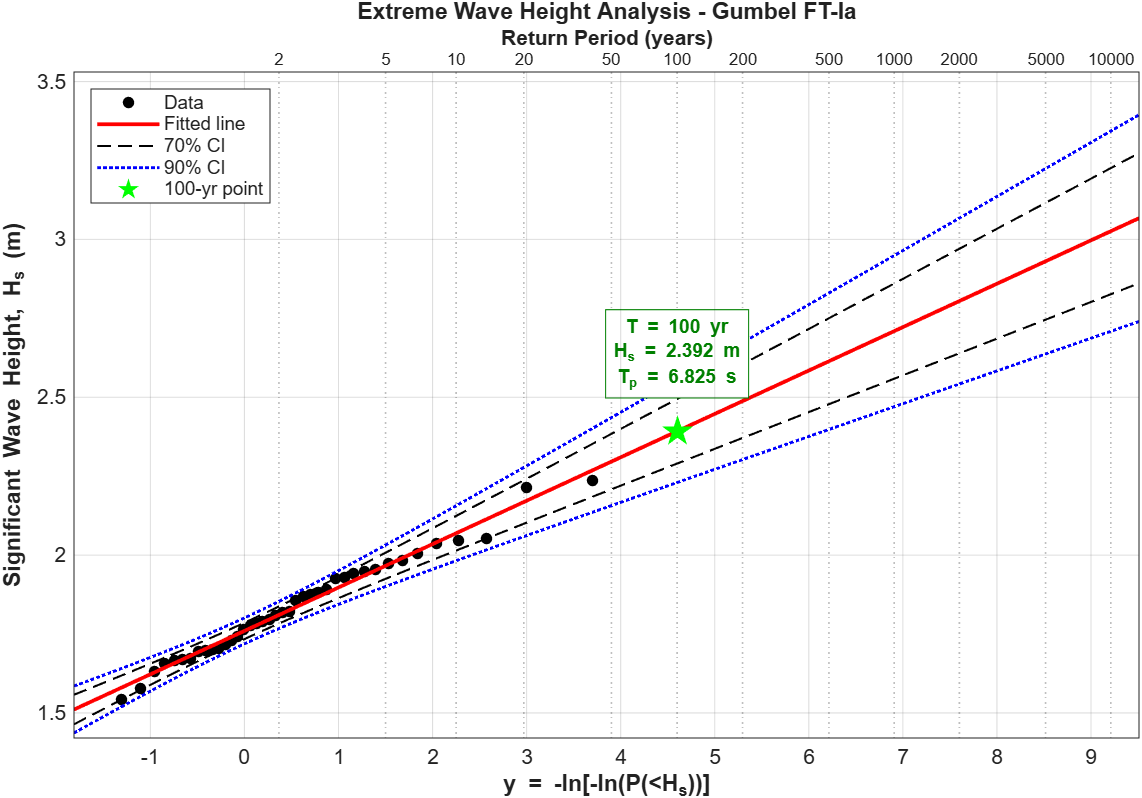
\includegraphics[width=0.74\textwidth]{gumbel_ft1a.png}
    \caption{Extreme wave height analysis based on the Gumbel FT-Ia distribution.}
    \label{fig:gumbel_ft1a}
\end{figure}

\begin{figure}[H]
    \centering
    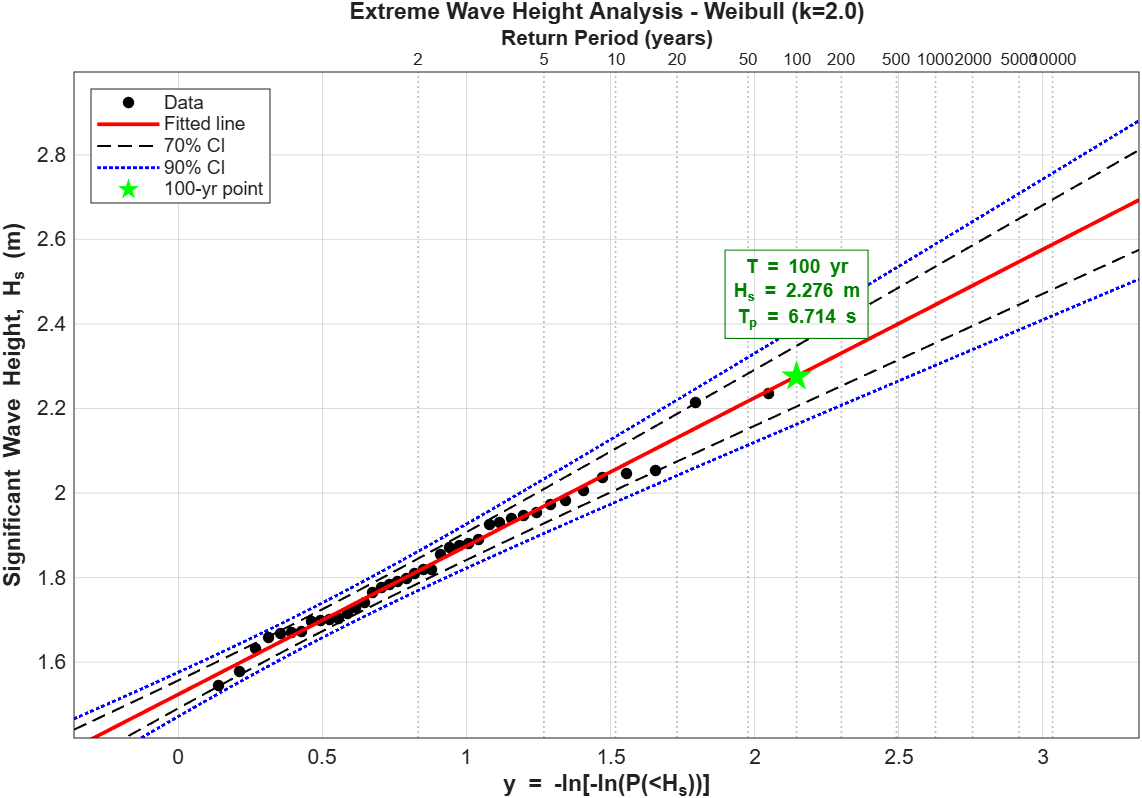
\includegraphics[width=0.74\textwidth]{weibull_k2.png}
    \caption{Extreme wave height analysis based on the Weibull \((k=2.0)\) distribution.}
    \label{fig:weibull_k2}
\end{figure}

Since the project definition requires the representative storm wind speed to be taken as the average wind speed during each storm, the results above were adopted as the main outcome of the study. However, in order to see how much the final estimate depends on this choice, a sensitivity check was also carried out using the maximum wind speed within each storm instead of the average value.

The effect of this change was significant. In the maximum-wind sensitivity case, the two top-ranked Gumbel distributions produced much larger 100-year wave heights than in the average-wind case. Gumbel FT-Ib gave \(H_s = 4.118\ \mathrm{m}\) and \(T_p = 8.278\ \mathrm{s}\), while Gumbel FT-Ia gave \(H_s = 4.198\ \mathrm{m}\) and \(T_p = 8.335\ \mathrm{s}\), as shown in Figures~\ref{fig:gumbel_ft1b_max} and~\ref{fig:gumbel_ft1a_max}. These values are much higher than the average-wind results and show that the estimated extreme wave height is highly sensitive to how each storm is represented in the hindcasting step.

This difference is expected. When the average storm wind is used, the wind forcing is smoothed over the whole storm duration, so short high-wind peaks do not control the result. When the maximum storm wind is used instead, the hindcast becomes much more peak-driven and the resulting annual maxima increase accordingly. For this reason, the maximum-wind case gives a useful upper-bound sensitivity check. However, the average-wind case is likely to provide a more realistic estimate of the extreme wave height at the site, since it accounts for the overall storm conditions rather than just short-term peaks.

\begin{figure}[H]
    \centering
    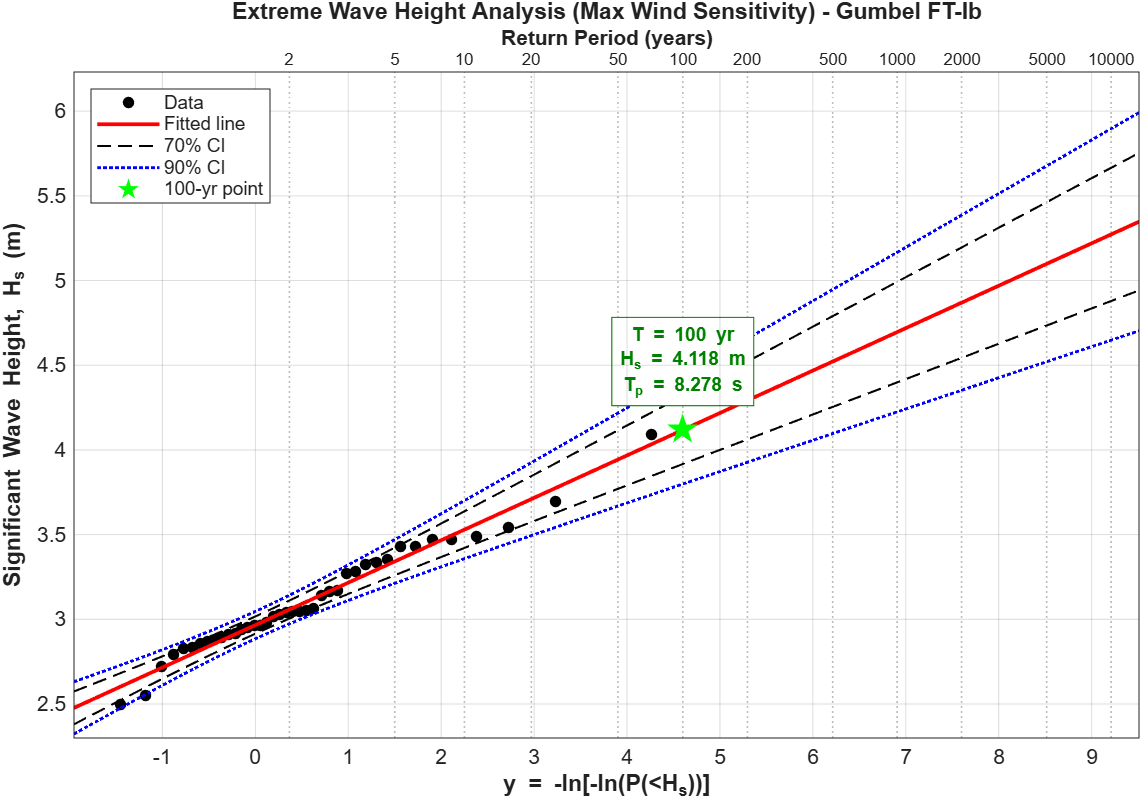
\includegraphics[width=0.72\textwidth]{gumbel_ft1b_maxwind_plot.png}
    \caption{Extreme wave height analysis based on the Gumbel FT-Ib distribution for the maximum-wind sensitivity case.}
    \label{fig:gumbel_ft1b_max}
\end{figure}

\begin{figure}[H]
    \centering
    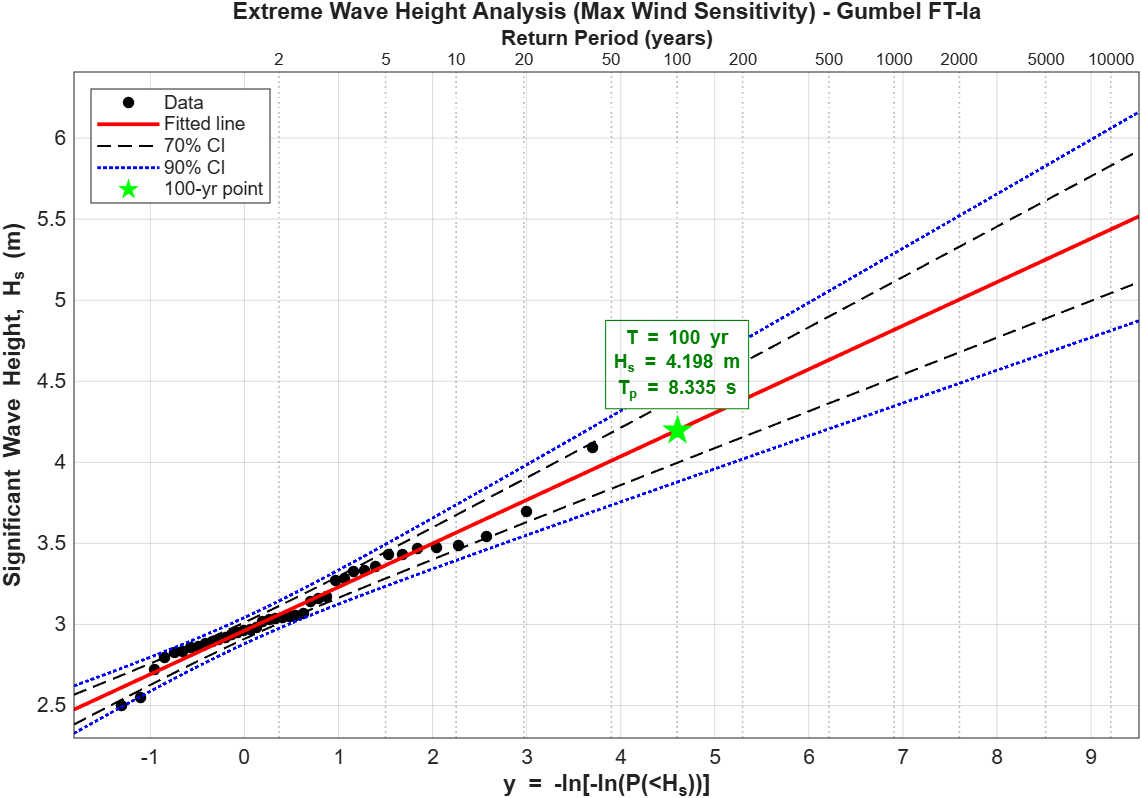
\includegraphics[width=0.72\textwidth]{gumbel_ft1a_maxwind_plot.png}
    \caption{Extreme wave height analysis based on the Gumbel FT-Ia distribution for the maximum-wind sensitivity case.}
    \label{fig:gumbel_ft1a_max}
\end{figure}

The long-term wave statistics obtained from the hourly wave height series are shown in Figure~\ref{fig:ltws}. From the fitted exceedance relation, the significant wave height exceeded for 10 hours per year was estimated as \(H_s = 2.308\ \mathrm{m}\), with a corresponding peak period of \(T_p = 7.041\ \mathrm{s}\). This value is very close to the 100-year return period wave height obtained from the average-wind extreme analysis. This result reflects the fetch-limited nature of the study area and the relatively narrow spread of the annual maxima series. In other words, the site can repeatedly experience severe wave conditions from the exposed sectors, but the enclosed basin geometry prevents the development of much larger open-sea wave heights.

\begin{figure}[H]
    \centering
    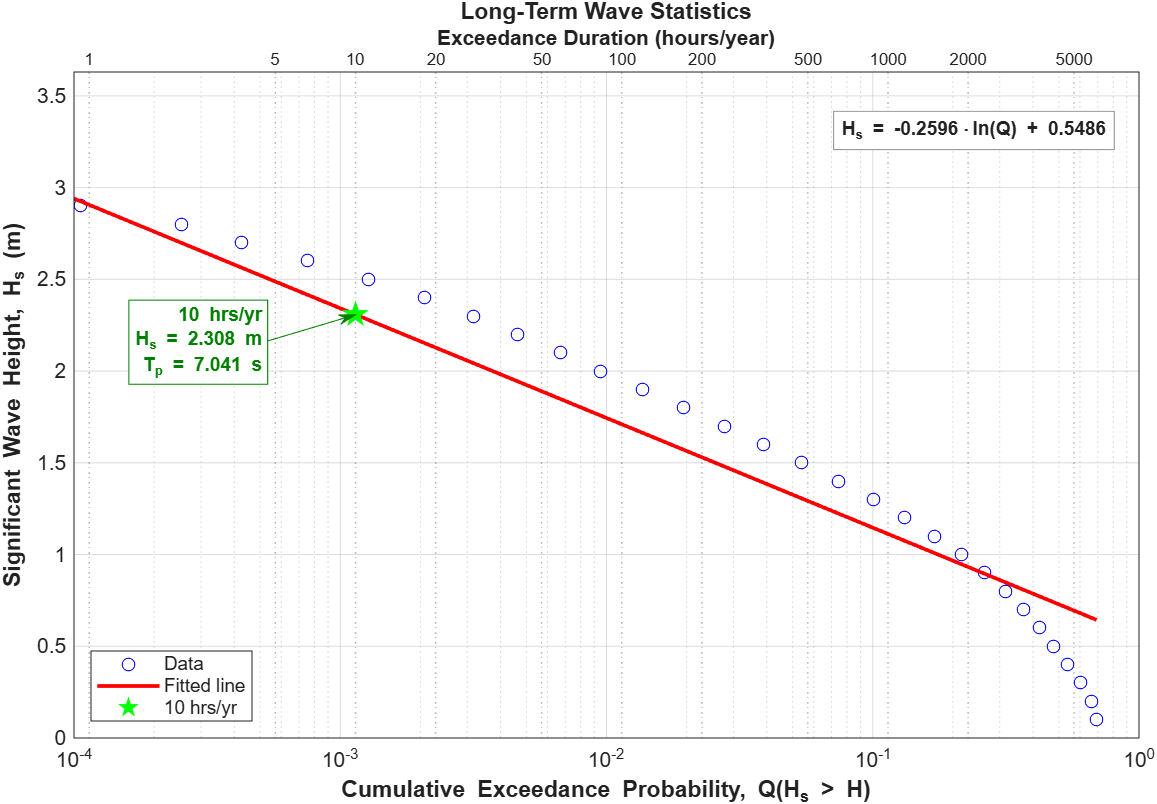
\includegraphics[width=0.69\textwidth]{ltws.png}
    \caption{Long-term wave statistics based on the hourly significant wave height series.}
    \label{fig:ltws}
\end{figure}

% -------------------- Conclusion --------------------
\section{Conclusion}

\hspace{0.5cm}In this study, the wind-wave climate of the Tekirdağ region in the Sea of Marmara was investigated using hourly ERA5 wind data for the period 1985--2024 at the offshore grid point \(40.75^\circ\mathrm{N}, 27.75^\circ\mathrm{E}\). Effective fetch lengths were calculated for the study point, the wind record was divided into individual storms, and significant wave heights and peak periods were hindcast using the JONSWAP method. Based on these results, both extreme wave analysis and long-term wave statistics were carried out.

The results showed that wave conditions at the study point are strongly controlled by directional fetch limitation. The largest storm and annual maximum wave heights were mainly associated with the \(E\), \(ENE\), and \(NE\) sectors, which correspond to the more exposed directions of the basin. The annual maxima remained within a relatively narrow range, which is consistent with the semi-enclosed nature of the Sea of Marmara and the limited wave growth potential at the site.

Among the candidate extreme value distributions tested, Gumbel FT-Ia gave the highest overall score based on the applied goodness-of-fit criteria. Using this distribution, the 100-year return period significant wave height was estimated as \(H_s = 2.392\ \mathrm{m}\), with a corresponding peak period of \(T_p = 6.825\ \mathrm{s}\). The long-term wave statistics analysis gave a significant wave height exceeded for 10 hours per year of \(H_s = 2.308\ \mathrm{m}\), with a corresponding peak period of \(T_p = 7.041\ \mathrm{s}\).

A sensitivity check based on maximum storm wind instead of average storm wind produced much larger extreme wave heights, showing that the final results are highly affected by how the representative storm wind is defined. However, the average-wind case is likely to provide a more realistic estimate of the extreme wave height at the site, since it accounts for the overall storm conditions rather than just short-term peaks.

Overall, the study shows that although the Tekirdağ offshore area does not allow the development of very large open-sea waves, it can still experience wave conditions that are important for coastal and port-related engineering assessment. The results obtained provide a site-specific description of the wave climate and can be used as a basis for further coastal engineering analyses in the region.
\newpage

% -------------------- References --------------------

\begin{thebibliography}{99}
\addcontentsline{toc}{section}{References}

\bibitem{}
Middle East Technical University, Department of Civil Engineering. (2025). \textit{CE 598 lecture notes} [Course notes].

\bibitem{}
Middle East Technical University, Department of Civil Engineering. (2025). \textit{CE 593 lecture notes} [Course notes].

\bibitem{}
European Centre for Medium-Range Weather Forecasts. (n.d.). \textit{ERA5 reanalysis}. https://www.ecmwf.int/

\bibitem{}
Wessel, P., \& Smith, W. H. F. (1996). A global self-consistent, hierarchical, high-resolution shoreline database. \textit{Journal of Geophysical Research: Solid Earth, 101}(B4), 8741--8743.

\bibitem{}
U.S. Army Corps of Engineers. (1984). \textit{Shore protection manual}.

\bibitem{}
Hasselmann, K., Barnett, T. P., Bouws, E., Carlson, H., Cartwright, D. E., Enke, K., Ewing, J. A., Gienapp, H., Hasselmann, D. E., Kruseman, P., Meerburg, A., M\"uller, P., Olbers, D. J., Richter, K., Sell, W., \& Walden, H. (1973). \textit{Measurements of wind-wave growth and swell decay during the Joint North Sea Wave Project (JONSWAP)}.

\end{thebibliography}
\newpage

% -------------------- Appendix --------------------
\appendix
\section{Appendix}

\subsection{Main MATLAB Code:}
\begin{lstlisting}[frame=single, numbers=left, style=Matlab-Pyglike]
clear; clc;
g = 9.81;

%% -------------------------
% SETTINGS
% -------------------------
wind_folder = 'era5_wind';
fetch_file  = 'Fetch_lengths.xlsx';

threshold = 3.0;   % storm threshold, m/s
iLat = 2;
iLon = 2;

run_maxU_sensitivity = true;   % sensitivity only

dirLabels16 = {'N','NNE','NE','ENE','E','ESE','SE','SSE', ...
               'S','SSW','SW','WSW','W','WNW','NW','NNW'};

%% -------------------------
% READ ALL YEARLY WIND FILES
% -------------------------
files = dir(fullfile(wind_folder, 'wind_*.nc'));
[~, idxSort] = sort({files.name});
files = files(idxSort);

U_all       = [];
windDir_all = [];
time_all    = [];

for i = 1:length(files)
    fpath = fullfile(wind_folder, files(i).name);

    u10_raw = ncread(fpath, 'u10');
    v10_raw = ncread(fpath, 'v10');
    t_raw   = ncread(fpath, 'valid_time');

    if i == 1
        lats = ncread(fpath, 'latitude');
        lons = ncread(fpath, 'longitude');
        fprintf('Using grid point: %.2fN, %.2fE\n', lats(iLat), lons(iLon));
    end

    u10 = squeeze(u10_raw(iLon, iLat, :));
    v10 = squeeze(v10_raw(iLon, iLat, :));

    U_all       = [U_all; sqrt(u10.^2 + v10.^2)];
    windDir_all = [windDir_all; mod(atan2d(-u10, -v10), 360)];
    time_all    = [time_all; datetime(1970,1,1) + seconds(t_raw)];
end

nHours = length(U_all);

%% -------------------------
% FETCH TABLE
% -------------------------
Tfetch = readtable(fetch_file);

fetchDir = mod(Tfetch.direction_deg, 360);
fetchLen = Tfetch.fetch_m;

[fetchDir, isrt] = sort(fetchDir);
fetchLen = fetchLen(isrt);

% 16-direction fetch values
fetch16 = fetchLen;

% Assign each hourly wind direction to one of the 16 bins
dirBin_hourly = mod(round(windDir_all / 22.5), 16) + 1;

% Use fetch directly from the corresponding bin
fetch_hourly = fetch16(dirBin_hourly);

%% -------------------------
% STORM DETECTION
% -------------------------
isStorm = U_all >= threshold;

stormStarts = find(diff([0; isStorm]) == 1);
stormEnds   = find(diff([isStorm; 0]) == -1);
nStorms     = length(stormStarts);

fprintf('Detected %d storms\n', nStorms);

%% -------------------------
% PER-STORM JONSWAP
% -------------------------
Hmo_hourly = zeros(nHours, 1);
Tp_hourly  = zeros(nHours, 1);

Hmo_storms = zeros(nStorms, 1);
Tp_storms  = zeros(nStorms, 1);

if run_maxU_sensitivity
    Hmo_storms_maxU = zeros(nStorms, 1);
    Tp_storms_maxU  = zeros(nStorms, 1);
end

dir_storms       = zeros(nStorms, 1);
year_storms      = zeros(nStorms, 1);
stormDuration_hr = zeros(nStorms, 1);
Uavg_storm       = zeros(nStorms, 1);
Umax_storm       = zeros(nStorms, 1);
FetchPeak_storm  = zeros(nStorms, 1);

for s = 1:nStorms
    idx        = stormStarts(s):stormEnds(s);
    Ustorm     = U_all(idx);
    Fstorm     = fetch_hourly(idx);
    storm_bins = dirBin_hourly(idx);

    U_avg = mean(Ustorm);
    U_max = max(Ustorm);
    t_dur = length(idx) * 3600;

    % Representative storm direction:
    % choose the bin with the largest fetch among bins present in the storm
    % if more than one bin has the same fetch, choose the most frequent one
    unique_bins   = unique(storm_bins);
    fetch_subset  = fetch16(unique_bins);
    max_fetch     = max(fetch_subset);
    candidate_bins = unique_bins(fetch_subset == max_fetch);

    if numel(candidate_bins) == 1
        rep_bin = candidate_bins;
    else
        counts = arrayfun(@(b) sum(storm_bins == b), candidate_bins);
        [~, imax] = max(counts);
        rep_bin = candidate_bins(imax);
    end

    peak_fetch = fetch16(rep_bin);
    peak_dir   = (rep_bin - 1) * 22.5;

    [Hmo_storms(s), Tp_storms(s)] = jonswap_basic(peak_fetch, U_avg, t_dur);

    % sensitivity only
    if run_maxU_sensitivity
        [Hmo_storms_maxU(s), Tp_storms_maxU(s)] = jonswap_basic(peak_fetch, U_max, t_dur);
    end

    dir_storms(s)       = peak_dir;
    year_storms(s)      = year(time_all(stormStarts(s)));
    stormDuration_hr(s) = length(idx);
    Uavg_storm(s)       = U_avg;
    Umax_storm(s)       = U_max;
    FetchPeak_storm(s)  = peak_fetch;

    % Hourly evolving wave calculation inside each storm
    for hi = 1:length(idx)
        h   = idx(hi);
        U_h = U_all(h);
        F_h = fetch_hourly(h);
        t_h = hi * 3600;

        if U_h > 0 && F_h > 0
            [Hmo_hourly(h), Tp_hourly(h)] = jonswap_basic(F_h, U_h, t_h);
        end
    end
end

%% -------------------------
% WAVE STEEPNESS
% -------------------------
Lp = g * Tp_storms.^2 / (2*pi);
steepness = Hmo_storms ./ Lp;

fprintf('Mean wave steepness: %.4f\n', mean(steepness));
fprintf('Max  wave steepness: %.4f\n', max(steepness));

%% -------------------------
% ANNUAL MAXIMA
% -------------------------
years_unique = unique(year_storms);
nYears       = length(years_unique);

ann_Hmo = zeros(nYears,1);
ann_Tp  = zeros(nYears,1);
ann_dir = zeros(nYears,1);

if run_maxU_sensitivity
    ann_Hmo_maxU = zeros(nYears,1);
    ann_Tp_maxU  = zeros(nYears,1);
    ann_dir_maxU = zeros(nYears,1);
end

for k = 1:nYears
    idx_yr = year_storms == years_unique(k);

    [ann_Hmo(k), i1] = max(Hmo_storms(idx_yr));
    tmpTp  = Tp_storms(idx_yr);
    tmpDir = dir_storms(idx_yr);
    ann_Tp(k)  = tmpTp(i1);
    ann_dir(k) = tmpDir(i1);

    if run_maxU_sensitivity
        [ann_Hmo_maxU(k), i2] = max(Hmo_storms_maxU(idx_yr));
        tmpTp2  = Tp_storms_maxU(idx_yr);
        tmpDir2 = dir_storms(idx_yr);
        ann_Tp_maxU(k)  = tmpTp2(i2);
        ann_dir_maxU(k) = tmpDir2(i2);
    end
end

ann_dir_labels = deg_to_16dir(ann_dir, dirLabels16);

AnnualMaxTable = table(years_unique, ann_Hmo, ann_Tp, string(ann_dir_labels(:)), ...
    'VariableNames', {'Year','Hs_annual_max_m','Tp_annual_max_s','Direction'});

%% -------------------------
% Hs-Tp RELATIONSHIPS
% -------------------------

% Extreme-analysis Tp model from annual maxima pairs
valid_ext = ann_Hmo > 0 & ann_Tp > 0;
pTp_ext = polyfit(log(ann_Hmo(valid_ext)), log(ann_Tp(valid_ext)), 1);
% Model form: Tp = exp(pTp_ext(2)) * Hs^(pTp_ext(1))

if run_maxU_sensitivity
    valid_ext_maxU = ann_Hmo_maxU > 0 & ann_Tp_maxU > 0;
    pTp_ext_maxU = polyfit(log(ann_Hmo_maxU(valid_ext_maxU)), log(ann_Tp_maxU(valid_ext_maxU)), 1);
end

% LTWS Tp model from hourly pairs
valid_hr = Hmo_hourly > 0 & Tp_hourly > 0;
pTp_hr = polyfit(log(Hmo_hourly(valid_hr)), log(Tp_hourly(valid_hr)), 1);
% Model form: Tp = exp(pTp_hr(2)) * Hs^(pTp_hr(1))

%% -------------------------
% EXTREME WAVE ANALYSIS
% -------------------------
v = 1;
dists = get_distributions(v);

% Average storm wind
[results, ScoreTable, sort_idx] = run_extreme_analysis(ann_Hmo, nYears, dists, v);

disp(ScoreTable)

plot_extreme_results(results, sort_idx, dists, ann_Hmo, nYears, v, pTp_ext, ...
    'Extreme Wave Height Analysis', '');

% Sensitivity case: maximum storm wind
if run_maxU_sensitivity
    [results_maxU, ~, sort_idx_maxU] = run_extreme_analysis(ann_Hmo_maxU, nYears, dists, v);

    plot_extreme_results(results_maxU, sort_idx_maxU, dists, ann_Hmo_maxU, nYears, v, pTp_ext_maxU, ...
        'Extreme Wave Height Analysis (Max Wind Sensitivity)', ' - max wind');
end

%% -------------------------
% LONG-TERM WAVE ANALYSIS
% -------------------------
bin_width = 0.1;
bin_edges = 0:bin_width:ceil(max(Hmo_hourly)*10)/10 + bin_width;
bin_lower = bin_edges(1:end-1)';
nBins     = length(bin_lower);

cum_freq = zeros(nBins,1);

for m = 1:nBins
    cum_freq(m) = sum(Hmo_hourly >= bin_lower(m));
end

Q = cum_freq / nHours;

valid   = Q > 0 & bin_lower > 0;
H_valid = bin_lower(valid);
Q_valid = Q(valid);

p         = polyfit(log(Q_valid), H_valid, 1);
A_over_23 = p(1);
B_LT      = p(2);

Q_10hr   = 10 / (365.25 * 24);
Hmo_10hr = A_over_23 * log(Q_10hr) + B_LT;
Tp_10hr = exp(polyval(pTp_hr, log(Hmo_10hr)));

fprintf('Eq: Hs = %.4f ln(Q) + %.4f\n', A_over_23, B_LT);
fprintf('Hs at 10 hrs/yr = %.3f m\n', Hmo_10hr);

Q_plot     = logspace(log10(min(Q_valid)), log10(max(Q_valid)), 300);
H_plot     = A_over_23 * log(Q_plot) + B_LT;
H_max_plot = max(H_valid) * 1.10;

keep   = H_plot >= 0 & H_plot <= H_max_plot;
Q_plot = Q_plot(keep);
H_plot = H_plot(keep);

%% -------------------------
% LONG-TERM WAVE PLOT
% -------------------------

T_hr_ticks = [1, 5, 10, 20, 50, 100, 200, 500, 1000, 2000, 5000];
Q_hr_ticks = T_hr_ticks / (365.25 * 24);

figure('Name', 'Long-Term Wave Statistics', 'WindowStyle', 'docked');
ax1 = axes('Position', [0.09 0.08 0.86 0.80]);
hold(ax1,'on'); box(ax1,'on');

yl = [0, H_max_plot];

for k = 1:length(Q_hr_ticks)
    plot(ax1, [Q_hr_ticks(k) Q_hr_ticks(k)], yl, ':', ...
        'Color',[0.75 0.75 0.75], 'LineWidth',0.7, 'HandleVisibility','off');
end

h1 = semilogx(ax1, Q_valid, H_valid, 'bo', 'MarkerSize',6, 'MarkerFaceColor','w');
h2 = semilogx(ax1, Q_plot, H_plot, 'r-', 'LineWidth',1.8);
h3 = semilogx(ax1, Q_10hr, Hmo_10hr, 'gp', 'MarkerFaceColor','g', 'MarkerSize',12);

ylim(ax1, yl);
xlim(ax1, [1e-4, 1]);
ax1.XScale  = 'log';
ax1.Layer   = 'top';
ax1.TickDir = 'none';

grid(ax1,'on');
xlabel(ax1, 'Cumulative Exceedance Probability, Q(H_s > H)', 'FontWeight','bold');
ylabel(ax1, 'Significant Wave Height, H_s (m)', 'FontWeight','bold');
legend(ax1, [h1 h2 h3], 'Data', 'Fitted line', '10 hrs/yr', 'Location','southwest');

text(ax1, 0.97, 0.93, ...
    sprintf('H_s = %.4f\\cdotln(Q) + %.4f', A_over_23, B_LT), ...
    'Units','normalized', 'HorizontalAlignment','right', 'VerticalAlignment','top', ...
    'FontSize',9, 'FontWeight','bold', 'BackgroundColor','white', ...
    'EdgeColor',[0.6 0.6 0.6]);

ax2 = axes('Position', ax1.Position, ...
    'XAxisLocation','top', 'YAxisLocation','right', ...
    'Color','none', 'YTick',[], 'YTickLabel',{}, 'XScale','log');
xlim(ax2, [1e-4, 1]);
ax2.XTick      = Q_hr_ticks;
ax2.XTickLabel = arrayfun(@num2str, T_hr_ticks, 'UniformOutput', false);
ax2.TickDir    = 'none';
ax2.FontSize   = 8;
ax2.XLabel.String   = 'Exceedance Duration (hours/year)';
ax2.XLabel.FontSize = 10;
ax2.XLabel.FontWeight = 'bold';

linkaxes([ax1 ax2],'x');
title(ax2, 'Long-Term Wave Statistics', 'FontSize',11, 'FontWeight','bold');

xr = xlim(ax1); yr = ylim(ax1); ap = ax1.Position;
xn = @(x) ap(1) + ap(3)*(log10(x)-log10(xr(1)))/(log10(xr(2))-log10(xr(1)));
yn = @(y) ap(2) + ap(4)*(y-yr(1))/diff(yr);

annotation(gcf,'textarrow', ...
    [xn(Q_10hr*0.45) xn(Q_10hr)], [yn(Hmo_10hr-0.15) yn(Hmo_10hr)], ...
    'String', sprintf('10 hrs/yr\nH_s = %.3f m\nT_p = %.3f s', Hmo_10hr, Tp_10hr), ...
    'FontSize',9, 'FontWeight','bold', 'Color',[0 0.5 0], ...
    'TextBackgroundColor','white', 'TextEdgeColor',[0 0.5 0], ...
    'HeadStyle','vback2', 'HeadLength',8, 'HeadWidth',6);

%% -------------------------
% EWTS FUNCTIONS
% -------------------------

function [results, ScoreTable, sort_idx] = run_extreme_analysis(ann_Hmo_in, nYears, dists, v)

    Hs_desc = sort(ann_Hmo_in, 'descend');
    Hs_asc  = sort(ann_Hmo_in);
    i = (1:nYears)';

    results = struct([]);

    for j = 1:10
        k    = dists(j).k;
        a_pp = dists(j).a_pp;
        b_pp = dists(j).b_pp;

        Fi = 1 - (i - a_pp) ./ (nYears + b_pp);

        if j == 1 || j == 2
            y = -log(-log(Fi));
        elseif j >= 3 && j <= 6
            y = (-log(Fi)).^(-1/k) - 1;
        else
            y = (-log(1 - Fi)).^(1/k);
        end

        x     = Hs_desc;
        Ybar  = mean(y);
        Xbar  = mean(x);
        VarY  = mean((y - Ybar).^2);
        VarX  = mean((x - Xbar).^2);
        CovYX = mean((y - Ybar) .* (x - Xbar));

        A = CovYX / VarY;
        B = Xbar - A * Ybar;

        if j == 1 || j == 2
            Fx = exp(-exp(-(Hs_asc - B) / A));
        elseif j >= 3 && j <= 6
            Fx = exp(-(1 + (Hs_asc - B) ./ (k*A)).^(-k));
        else
            Fx = 1 - exp(-((Hs_asc - B) ./ A).^k);
        end

        r  = CovYX / sqrt(VarX * VarY);
        R2 = r^2;

        Delta_r     = 1 - r;
        Delta_rmean = exp(dists(j).a_MIR + dists(j).b_MIR*log(nYears) + dists(j).c_MIR*(log(nYears))^2);
        MIR         = Delta_r / Delta_rmean;

        x1   = Hs_desc(1);
        xbar = mean(Hs_desc);
        s    = std(Hs_desc, 1);
        xi   = (x1 - xbar) / s;

        xi95 = dists(j).a_DOL_95 + dists(j).b_DOL_95*log(nYears) + dists(j).c_DOL_95*(log(nYears))^2;
        xi5  = dists(j).a_DOL_5  + dists(j).b_DOL_5 *log(nYears) + dists(j).c_DOL_5 *(log(nYears))^2;
        pass_DOL = (xi > xi5) && (xi < xi95);

        Delta_r95 = exp(dists(j).a_REC + dists(j).b_REC*log(nYears) + dists(j).c_REC*(log(nYears))^2);
        pass_REC  = Delta_r < Delta_r95;

        S1      = (i - 1) / nYears;
        S2      = i / nYears;
        D_1     = Fx - S1;
        D_2     = S2 - Fx;
        D_KS    = max(max(D_1), max(D_2));
        pass_KS = D_KS < 0.24;

        results(j).name     = dists(j).name;
        results(j).A        = A;
        results(j).B        = B;
        results(j).R        = r;
        results(j).R2       = R2;
        results(j).MIR      = MIR;
        results(j).pass_REC = pass_REC;
        results(j).pass_DOL = pass_DOL;
        results(j).pass_KS  = pass_KS;
        results(j).y        = y;
    end

    % Build score table
    dist_names = {results.name}';
    R2_vals    = [results.R2]';
    MIR_vals   = [results.MIR]';

    [~, tmp] = sort(R2_vals, 'ascend');
    R2_pts = zeros(10,1); R2_pts(tmp) = 1:10;

    [~, tmp] = sort(MIR_vals, 'descend');
    MIR_pts = zeros(10,1); MIR_pts(tmp) = 1:10;

    REC_str = cell(10,1); REC_pts = zeros(10,1);
    DOL_str = cell(10,1); DOL_pts = zeros(10,1);
    KS_str  = cell(10,1); KS_pts  = zeros(10,1);

    for j = 1:10
        if results(j).pass_REC
            REC_str{j} = 'ACCEPTED'; REC_pts(j) = 10;
        else
            REC_str{j} = 'NOT ACCEPTED'; REC_pts(j) = 0;
        end

        if results(j).pass_DOL
            DOL_str{j} = 'ACCEPTED'; DOL_pts(j) = 10;
        else
            DOL_str{j} = 'NOT ACCEPTED'; DOL_pts(j) = 0;
        end

        if results(j).pass_KS
            KS_str{j} = 'ACCEPTED'; KS_pts(j) = 10;
        else
            KS_str{j} = 'NOT ACCEPTED'; KS_pts(j) = 0;
        end
    end

    total_pts = R2_pts + MIR_pts + REC_pts + DOL_pts + KS_pts;
    [~, tmp]  = sort(total_pts, 'descend');
    overall_rank = zeros(10,1);
    overall_rank(tmp) = 1:10;

    [~, sort_idx] = sort(overall_rank);

    ScoreTable = table(dist_names(sort_idx), ...
        R2_vals(sort_idx), MIR_vals(sort_idx), REC_str(sort_idx), DOL_str(sort_idx), KS_str(sort_idx), ...
        R2_pts(sort_idx), MIR_pts(sort_idx), REC_pts(sort_idx), DOL_pts(sort_idx), KS_pts(sort_idx), ...
        total_pts(sort_idx), ...
        'VariableNames', {'Distribution','R2','MIR','REC','DOL','KS', ...
                          'Score_R2','Score_MIR','Score_REC','Score_DOL','Score_KS','Total'});
end

function plot_extreme_results(results, sort_idx, dists, ann_Hmo_in, nYears, v, pTp_ext, baseTitle, nameSuffix)

    Hs_desc = sort(ann_Hmo_in, 'descend');

    top2_idx = sort_idx(1:2);

    T_ticks = [2, 5, 10, 20, 50, 100, 200, 500, 1000, 2000, 5000, 10000];
    F_ticks = 1 - 1./T_ticks;

    for p = 1:2
        j = top2_idx(p);
        d = results(j);
        k = dists(j).k;

        if j <= 2
            y_ticks = -log(-log(F_ticks));
            y_100   = -log(-log(1 - 1/100));
        elseif j <= 6
            y_ticks = (-log(F_ticks)).^(-1/k) - 1;
            y_100   = (-log(1-1/100))^(-1/k) - 1;
        else
            y_ticks = (-log(1 - F_ticks)).^(1/k);
            y_100   = (-log(1/100))^(1/k);
        end

        y_min  = min(d.y) - 0.5;
        y_max  = max(y_ticks) + 0.3;
        y_plot = linspace(y_min, y_max, 200);

        x_fit  = d.A * y_plot + d.B;
        Hmo_100 = d.A * y_100 + d.B;
        Tp_100 = exp(polyval(pTp_ext, log(Hmo_100)));

        sigma_x = sqrt((1/nYears) * sum((Hs_desc - mean(Hs_desc)).^2));
        a_cb    = dists(j).a1 * exp(dists(j).a2*nYears^(-1.3) + dists(j).kappa*(-log(v))^2);
        sigma_z = sqrt(1 + a_cb*(y_plot - dists(j).c + dists(j).alpha_cb*log(v)).^2) / sqrt(nYears);
        sigma_X = sigma_z * sigma_x;

        z70 = norminv(0.85);
        z90 = norminv(0.95);

        x70U = x_fit + z70*sigma_X;
        x70L = x_fit - z70*sigma_X;
        x90U = x_fit + z90*sigma_X;
        x90L = x_fit - z90*sigma_X;

        figure('Name', [dists(j).name nameSuffix], 'WindowStyle', 'docked');
        ax1 = axes('Position', [0.09 0.08 0.86 0.80]);
        hold(ax1,'on'); box(ax1,'on');

        yl = [min(Hs_desc)*0.92, max(x90U)*1.04];

        for t = 1:length(y_ticks)
            plot(ax1, [y_ticks(t) y_ticks(t)], yl, ':', ...
                'Color',[0.75 0.75 0.75], 'LineWidth',0.8, 'HandleVisibility','off');
        end

        h1 = plot(ax1, d.y, Hs_desc, 'ko', 'MarkerFaceColor','k', 'MarkerSize',5);
        h2 = plot(ax1, y_plot, x_fit, 'r-', 'LineWidth',1.8);
        h3 = plot(ax1, y_plot, x70U, 'k--', 'LineWidth',1.0);
             plot(ax1, y_plot, x70L, 'k--', 'LineWidth',1.0, 'HandleVisibility','off');
        h4 = plot(ax1, y_plot, x90U, 'b:', 'LineWidth',1.4);
             plot(ax1, y_plot, x90L, 'b:', 'LineWidth',1.4, 'HandleVisibility','off');
        h5 = plot(ax1, y_100, Hmo_100, 'p', ...
            'MarkerFaceColor','g', 'MarkerEdgeColor','g', 'MarkerSize',14);

        [~, i100] = min(abs(y_plot - y_100));
        text(ax1, y_100, max(x90U(i100), Hmo_100) + 0.08, ...
            sprintf('T = 100 yr\nH_s = %.3f m\nT_p = %.3f s', Hmo_100, Tp_100), ...
            'FontSize', 9, 'Color', [0 0.5 0], 'FontWeight', 'bold', ...
            'HorizontalAlignment', 'center', ...
            'BackgroundColor', 'white', 'EdgeColor', [0 0.5 0]);

        ylim(ax1, yl);
        xlim(ax1, [y_min, y_max]);
        xlabel(ax1, 'y = -ln[-ln(P(<H_s))]', 'FontWeight', 'bold');
        ylabel(ax1, 'Significant Wave Height, H_s (m)', 'FontWeight', 'bold');
        legend(ax1, [h1 h2 h3 h4 h5], 'Data','Fitted line','70% CI','90% CI','100-yr point', ...
            'Location','northwest');
        grid(ax1,'on');
        ax1.TickDir = 'none';
        ax1.Layer   = 'top';

        ax2 = axes('Position', ax1.Position, ...
            'XAxisLocation','top', 'YAxisLocation','right', ...
            'Color','none', 'YTick',[], 'YTickLabel',{});
        xlim(ax2, [y_min, y_max]);
        ax2.XTick      = y_ticks;
        ax2.XTickLabel = arrayfun(@num2str, T_ticks, 'UniformOutput', false);
        ax2.TickDir    = 'none';
        ax2.FontSize   = 8;
        ax2.XLabel.String = 'Return Period (years)';
        ax2.XLabel.FontSize = 10;
        ax2.XLabel.FontWeight = 'bold';

        linkaxes([ax1 ax2],'x');

        title(ax2, sprintf('%s - %s', baseTitle, dists(j).name), ...
            'FontSize', 11, 'FontWeight', 'bold');
    end
end

%% -------------------------
% JONSWAP FUNCTION
% -------------------------
function [H_s, T_p] = jonswap_basic(fetch, U_input, t_duration)

    g = 9.81;
    U_A = 0.71 * U_input^1.23;

    F_star = g * fetch / (U_A^2);
    t_star = g * t_duration / U_A;

    H_s_star_FD = 0.243;
    T_p_star_FD = 8.13;

    H_s_FD = H_s_star_FD * U_A^2 / g;
    T_p_FD = T_p_star_FD * U_A / g;

    F_star_eff = (t_star / 68.8)^(3/2);
    F_eff = min(F_star, F_star_eff);

    H_s_star_D = 0.0016 * F_eff^(1/2);
    T_p_star_D = 0.286  * F_eff^(1/3);

    H_s_D = H_s_star_D * U_A^2 / g;
    T_p_D = T_p_star_D * U_A / g;

    H_s = min(H_s_FD, H_s_D);
    T_p = min(T_p_FD, T_p_D);
end

%% -------------------------
% DEGREE TO 16-SECTOR LABEL
% -------------------------
function labels = deg_to_16dir(degVals, dirLabels16)
    idx = mod(round(degVals / 22.5), 16) + 1;
    labels = dirLabels16(idx);
end

%% -------------------------
% TOP 10 STORMS TABLE
% -------------------------
storm_dir_labels = deg_to_16dir(dir_storms, dirLabels16);

TopStormTable = table(year_storms, stormDuration_hr, Umax_storm, string(storm_dir_labels(:)), ...
    FetchPeak_storm/1000, Hmo_storms, Tp_storms, ...
    'VariableNames', {'Year','Duration_hr','Umax_mps','Direction','PeakFetch_km','Hs_m','Tp_s'});

[~, stormSortIdx] = sort(TopStormTable.Hs_m, 'descend');
TopStormTable = TopStormTable(stormSortIdx(1:min(10,height(TopStormTable))), :);

disp(AnnualMaxTable)
disp(ScoreTable)
disp(TopStormTable)

%% -------------------------
% LATEX EXPORTS
% -------------------------
write_annual_maxima_tex('Annual_Maxima_Table.tex', years_unique, ann_Hmo, ann_Tp, ann_dir_labels);
write_top10_storms_tex('Top10_Storms_Table.tex', TopStormTable);
write_score_table_tex('Score_Table.tex', ScoreTable);

%% -------------------------
% LATEX TABLE EXPORT HELPERS
% -------------------------

function write_annual_maxima_tex(filename, years_unique, ann_Hmo, ann_Tp, ann_dir_labels)

    fid = fopen(filename, 'w');
    if fid == -1
        error('Could not open %s for writing.', filename);
    end

    fprintf(fid, '\\begin{tabular}{cccc}\n');
    fprintf(fid, '\\hline\n');
    fprintf(fid, 'Year & $H_s$ (m) & $T_p$ (s) & Direction \\\\\n');
    fprintf(fid, '\\hline\n');

    for i = 1:numel(years_unique)
        fprintf(fid, '%d & %.3f & %.3f & %s \\\\\n', ...
            years_unique(i), ann_Hmo(i), ann_Tp(i), char(ann_dir_labels(i)));
    end

    fprintf(fid, '\\hline\n');
    fprintf(fid, '\\end{tabular}\n');
    fclose(fid);
end


function write_top10_storms_tex(filename, TopStormTable)

    fid = fopen(filename, 'w');
    if fid == -1
        error('Could not open %s for writing.', filename);
    end

    fprintf(fid, '\\begin{tabular}{ccccccc}\n');
    fprintf(fid, '\\hline\n');
    fprintf(fid, 'Year & Duration (hr) & $U_{max}$ (m/s) & Direction & Peak Fetch (km) & $H_s$ (m) & $T_p$ (s) \\\\\n');
    fprintf(fid, '\\hline\n');

    for i = 1:height(TopStormTable)
        fprintf(fid, '%d & %d & %.3f & %s & %.3f & %.3f & %.3f \\\\\n', ...
            round(TopStormTable.Year(i)), ...
            round(TopStormTable.Duration_hr(i)), ...
            TopStormTable.Umax_mps(i), ...
            char(TopStormTable.Direction(i)), ...
            TopStormTable.PeakFetch_km(i), ...
            TopStormTable.Hs_m(i), ...
            TopStormTable.Tp_s(i));
    end

    fprintf(fid, '\\hline\n');
    fprintf(fid, '\\end{tabular}\n');
    fclose(fid);
end


function write_score_table_tex(filename, ScoreTable)

    fid = fopen(filename, 'w');
    if fid == -1
        error('Could not open %s for writing.', filename);
    end

    fprintf(fid, '\\small\n');
    fprintf(fid, '\\resizebox{\\textwidth}{!}{%%\n');
    fprintf(fid, '\\begin{tabular}{|l|c|c|c|c|c||c|c|c|c|c|c|}\n');
    fprintf(fid, '\\hline\n');
    fprintf(fid, '\\multicolumn{6}{|c||}{} & \\multicolumn{6}{c|}{\\textbf{SCORE}} \\\\ \\hline\n');
    fprintf(fid, 'Distribution & $R^2$ & MIR & REC & DOL & KS & $R^2$ & MIR & REC & DOL & KS & Total \\\\ \\hline\n');

    for i = 1:height(ScoreTable)
        dist = char(ScoreTable.Distribution(i));
        dist = strrep(dist, '(k=', '($k=');
        dist = strrep(dist, ')', '$)');

        fprintf(fid, '%s & %.4f & %.4f & %s & %s & %s & %d & %d & %d & %d & %d & %d \\\\ \\hline\n', ...
            dist, ...
            ScoreTable.R2(i), ...
            ScoreTable.MIR(i), ...
            char(ScoreTable.REC(i)), ...
            char(ScoreTable.DOL(i)), ...
            char(ScoreTable.KS(i)), ...
            round(ScoreTable.Score_R2(i)), ...
            round(ScoreTable.Score_MIR(i)), ...
            round(ScoreTable.Score_REC(i)), ...
            round(ScoreTable.Score_DOL(i)), ...
            round(ScoreTable.Score_KS(i)), ...
            round(ScoreTable.Total(i)));
    end

    fprintf(fid, '\\end{tabular}%%\n');
    fprintf(fid, '}\n');
    fclose(fid);
end

\end{lstlisting}

\subsection{Distribution Constants Helper Function:}
\begin{lstlisting}[frame=single, numbers=left, style=Matlab-Pyglike]
    function dists = get_distributions(v)
dists = struct();

% Gumbel FT-Ia
dists(1).name  = 'Gumbel FT-Ia';
dists(1).type  = 'gumbel';
dists(1).k     = NaN;

dists(1).a_pp  = 0;    % Plotting position alpha
dists(1).b_pp  = 1;    % Plotting position beta

dists(1).a1    = 0.64; dists(1).a2 = 9.0; 
dists(1).kappa = 0.93; dists(1).c  = 0; 
dists(1).alpha_cb = 1.33; % Sigma_z calculation

dists(1).a_MIR = -2.364 + 0.54*v^(5/2); 
dists(1).b_MIR = -0.2665 - 0.0457*v^(5/2);
dists(1).c_MIR = -0.044;    % MIR Criterion

dists(1).a_DOL_95 = -0.579 + 0.468*v; 
dists(1).b_DOL_95 = 1.496 - 0.227*v^2;
dists(1).c_DOL_95 = -0.038; % DOL Criterion 95%
dists(1).a_DOL_5 = 0.257 + 0.133*v^2; 
dists(1).b_DOL_5 = 0.452 - 0.118*v^2;
dists(1).c_DOL_5 = 0.032;   % DOL Criterion 5%

dists(1).a_REC = -1.444; dists(1).b_REC = -0.2733 - 0.0414*v^(5/2);
dists(1).c_REC = -0.045;    % REC Criterion

% Gumbel FT-Ib
dists(2).name  = 'Gumbel FT-Ib';
dists(2).type  = 'gumbel';
dists(2).k     = NaN;

dists(2).a_pp  = 0.44;
dists(2).b_pp  = 0.12;

dists(2).a1    = 0.64;  dists(2).a2 = 9.0;
dists(2).kappa = 0.93;  dists(2).c  = 0; 
dists(2).alpha_cb = 1.33;

dists(2).a_MIR = -2.364 + 0.54*v^(5/2);
dists(2).b_MIR = -0.2665 - 0.0457*v^(5/2);
dists(2).c_MIR = -0.044;

dists(2).a_DOL_95 = -0.579 + 0.468*v; 
dists(2).b_DOL_95 = 1.496 - 0.227*v^2; 
dists(2).c_DOL_95 = -0.038;
dists(2).a_DOL_5  = 0.257 + 0.133*v^2; 
dists(2).b_DOL_5  = 0.452 - 0.118*v^2; 
dists(2).c_DOL_5  = 0.032;

dists(2).a_REC = -1.444;
dists(2).b_REC = -0.2733 - 0.0414*v^(5/2);
dists(2).c_REC = -0.045;

% FT-II k=2.5
dists(3).name  = 'FT-II (k=2.5)';
dists(3).type  = 'ft2';
dists(3).k     = 2.5;

dists(3).a_pp  = 0.44 + 0.52/2.5;
dists(3).b_pp  = 0.12 - 0.11/2.5;

dists(3).a1    = 1.27;  dists(3).a2  = 0.12;
dists(3).kappa = 0.24;  dists(3).c   = 0.3; 
dists(3).alpha_cb = 2.3; dists(3).N0 = 23;
dists(3).v0 = 1.34;

dists(3).a_MIR = -2.470 + 0.015*v^(3/2);
dists(3).b_MIR = -0.1530 - 0.0052*v^(5/2);
dists(3).c_MIR = 0;

dists(3).a_DOL_95 = 4.653 - 1.076*v^(1/2);  
dists(3).b_DOL_95 = -2.047 + 0.307*v^(1/2); 
dists(3).c_DOL_95 = 0.635;
dists(3).a_DOL_5  = 1.481 - 0.126*v^(1/4);  
dists(3).b_DOL_5  = -0.331 - 0.031*v^2;     
dists(3).c_DOL_5  = 0.192;

dists(3).a_REC = -1.122 - 0.037*v;
dists(3).b_REC = -0.3298 + 0.0105*v^(1/4);
dists(3).c_REC = 0.016;

% FT-II k=3.33
dists(4).name  = 'FT-II (k=3.33)';
dists(4).type  = 'ft2';
dists(4).k     = 3.33;

dists(4).a_pp  = 0.44 + 0.52/3.33;
dists(4).b_pp  = 0.12 - 0.11/3.33;
dists(4).a1    = 1.23;  dists(4).a2  = 0.09;
dists(4).kappa = 0.36;  dists(4).c   = 0.2;  
dists(4).alpha_cb = 1.9; dists(4).N0 = 25;    
dists(4).v0 = 0.66;

dists(4).a_MIR = -2.462 - 0.009*v^2;
dists(4).b_MIR = -0.1933 - 0.0037*v^(5/2);
dists(4).c_MIR = -0.007;

dists(4).a_DOL_95 = 3.217 - 1.216*v^(1/4);  
dists(4).b_DOL_95 = -0.903 + 0.294*v^(1/4); 
dists(4).c_DOL_95 = 0.427;
dists(4).a_DOL_5  = 1.025;                   
dists(4).b_DOL_5  = -0.077 - 0.050*v^2;      
dists(4).c_DOL_5  = 0.143;

dists(4).a_REC = -1.306 - 0.105*v^(3/2);
dists(4).b_REC = -0.3001 + 0.0404*v^(1/2);
dists(4).c_REC = 0;

% FT-II k=5.0
dists(5).name  = 'FT-II (k=5.0)';
dists(5).type  = 'ft2';
dists(5).k     = 5.0;

dists(5).a_pp  = 0.44 + 0.52/5.0;
dists(5).b_pp  = 0.12 - 0.11/5.0;
dists(5).a1    = 1.34;  dists(5).a2  = 0.07;
dists(5).kappa = 0.41;  dists(5).c   = 0.1;  
dists(5).alpha_cb = 1.6; dists(5).N0 = 35;    
dists(5).v0 = 0.45;

dists(5).a_MIR = -2.463;
dists(5).b_MIR = -0.2110 - 0.0131*v^(5/2);
dists(5).c_MIR = -0.019;

dists(5).a_DOL_95 = 0.599 - 0.038*v^2;      
dists(5).b_DOL_95 = 0.518 - 0.045*v^2;      
dists(5).c_DOL_95 = 0.210;
dists(5).a_DOL_5  = 0.700 + 0.060*v^2;      
dists(5).b_DOL_5  = 0.139 - 0.076*v^2;      
dists(5).c_DOL_5  = 0.100;

dists(5).a_REC = -1.463 - 0.107*v^(3/2);
dists(5).b_REC = -0.2716 + 0.0517*v^(1/4);
dists(5).c_REC = -0.018;

% FT-II k=10.0
dists(6).name  = 'FT-II (k=10.0)';
dists(6).type  = 'ft2';
dists(6).k     = 10.0;

dists(6).a_pp  = 0.44 + 0.52/10.0;
dists(6).b_pp  = 0.12 - 0.11/10.0;

dists(6).a1    = 1.48;  dists(6).a2  = 0.06;
dists(6).kappa = 0.47;  dists(6).c   = 0;   
dists(6).alpha_cb = 1.4; dists(6).N0 = 60;    
dists(6).v0 = 0.34;

dists(6).a_MIR = -2.437 + 0.028*v^(5/2);
dists(6).b_MIR = -0.2280 - 0.0300*v^(5/2);
dists(6).c_MIR = -0.033;

dists(6).a_DOL_95 = -0.371 + 0.171*v^2;     
dists(6).b_DOL_95 = 1.283 - 0.133*v^2;      
dists(6).c_DOL_95 = 0.045;
dists(6).a_DOL_5  = 0.424 + 0.088*v^2;      
dists(6).b_DOL_5  = 0.329 - 0.094*v^2;      
dists(6).c_DOL_5  = 0.061;

dists(6).a_REC = -1.490 - 0.073*v;
dists(6).b_REC = -0.2299 - 0.0099*v^(5/2);
dists(6).c_REC = -0.034;

% Weibull k=0.75
dists(7).name  = 'Weibull (k=0.75)';
dists(7).type  = 'weibull';
dists(7).k     = 0.75;

dists(7).a_pp  = 0.20 + 0.27/0.75^0.5;
dists(7).b_pp  = 0.20 + 0.23/0.75^0.5;
dists(7).a1    = 1.65;  dists(7).a2 = 11.4;
dists(7).kappa = -0.63; dists(7).c  = 0;    
dists(7).alpha_cb = 1.15;

dists(7).a_MIR = -2.435 - 0.168*v^(1/2);
dists(7).b_MIR = -0.2083 + 0.1074*v^(1/2);
dists(7).c_MIR = -0.047;

dists(7).a_DOL_95 = -0.256 - 0.632*v^2;     
dists(7).b_DOL_95 = 1.269 + 0.254*v^2;      
dists(7).c_DOL_95 = 0.037;
dists(7).a_DOL_5  = 0.534 - 0.162*v;        
dists(7).b_DOL_5  = 0.277 + 0.095*v;         
dists(7).c_DOL_5  = 0.065;

dists(7).a_REC = -1.473 - 0.049*v^2;
dists(7).b_REC = -0.2181 + 0.0505*v;
dists(7).c_REC = -0.041;

% Weibull k=1.0
dists(8).name  = 'Weibull (k=1.0)';
dists(8).type  = 'weibull';
dists(8).k     = 1.0;

dists(8).a_pp  = 0.20 + 0.27/1.0^0.5;
dists(8).b_pp  = 0.20 + 0.23/1.0^0.5;

dists(8).a1    = 1.92;  dists(8).a2 = 11.4;
dists(8).kappa = 0;     dists(8).c  = 0.3;  
dists(8).alpha_cb = 0.90;

dists(8).a_MIR = -2.355;
dists(8).b_MIR = -0.2612;
dists(8).c_MIR = -0.043;

dists(8).a_DOL_95 = -0.682;                  
dists(8).b_DOL_95 = 1.600;                   
dists(8).c_DOL_95 = -0.045;
dists(8).a_DOL_5  = 0.308;                   
dists(8).b_DOL_5  = 0.423;                   
dists(8).c_DOL_5  = 0.037;

dists(8).a_REC = -1.433;
dists(8).b_REC = -0.2679;
dists(8).c_REC = -0.044;

% Weibull k=1.4
dists(9).name  = 'Weibull (k=1.4)';
dists(9).type  = 'weibull';
dists(9).k     = 1.4;

dists(9).a_pp  = 0.20 + 0.27/1.4^0.5;
dists(9).b_pp  = 0.20 + 0.23/1.4^0.5;

dists(9).a1    = 2.05;  dists(9).a2 = 11.4;
dists(9).kappa = 0.69;  dists(9).c  = 0.4;  
dists(9).alpha_cb = 0.72;

dists(9).a_MIR = -2.277 + 0.056*v^(1/2);
dists(9).b_MIR = -0.3169 - 0.0499*v;
dists(9).c_MIR = -0.044;

dists(9).a_DOL_95 = -0.548 + 0.452*v^(1/2); 
dists(9).b_DOL_95 = 1.521 - 0.184*v;        
dists(9).c_DOL_95 = -0.065;
dists(9).a_DOL_5  = 0.192 + 0.126*v^(3/2);  
dists(9).b_DOL_5  = 0.501 - 0.081*v^(3/2);  
dists(9).c_DOL_5  = 0.018;

dists(9).a_REC = -1.312;
dists(9).b_REC = -0.3356 - 0.0449*v;
dists(9).c_REC = -0.045;

% Weibull k=2.0
dists(10).name  = 'Weibull (k=2.0)';
dists(10).type  = 'weibull';
dists(10).k     = 2.0;

dists(10).a_pp  = 0.20 + 0.27/2.0^0.5;
dists(10).b_pp  = 0.20 + 0.23/2.0^0.5;

dists(10).a1    = 2.24;  dists(10).a2 = 11.4;
dists(10).kappa = 1.34;  dists(10).c  = 0.5;  
dists(10).alpha_cb = 0.54;

dists(10).a_MIR = -2.160 + 0.113*v;
dists(10).b_MIR = -0.3788 - 0.0979*v;
dists(10).c_MIR = -0.041;

dists(10).a_DOL_95 = -0.322 + 0.641*v^(1/2); 
dists(10).b_DOL_95 = 1.414 - 0.326*v;       
dists(10).c_DOL_95 = -0.069;
dists(10).a_DOL_5  = 0.050 + 0.182*v^(3/2);  
dists(10).b_DOL_5  = 0.592 - 0.139*v^(3/2); 
dists(10).c_DOL_5  = 0;

dists(10).a_REC = -1.188 + 0.073*v^(1/2);
dists(10).b_REC = -0.4401 - 0.0846*v^(3/2);
dists(10).c_REC = -0.039;
\end{lstlisting}

\subsection{Fetch Calculation Python Code:}
\begin{lstlisting}[frame=single, numbers=left, language=Python, basicstyle=\ttfamily\scriptsize\small\color{black}]
"""
SPM Effective Fetch Calculator (+-42deg Method)

Author: Bilge Evran

-------------------------------------------
SETUP INSTRUCTIONS
-------------------------------------------

1) Install required Python packages:

pip install os numpy matplotlib pandas geopandas shapely pyproj openpyxl

2) Download the GSHHG coastline dataset manually:

https://www.ngdc.noaa.gov/mgg/shorelines/data/gshhg/latest/gshhg-shp-2.3.7.zip

3) Extract the ZIP file.

Your folder structure should look like this:

project_folder/
 |
 |-- fetch_calculator.py
 `-- gshhg-shp-2.3.7/
     `-- GSHHS_shp/
         `-- f/
             `-- GSHHS_f_L1.shp

4) Update the path below if necessary.
"""

import os
import numpy as np
import pandas as pd
import geopandas as gpd
import matplotlib.pyplot as plt
from shapely.geometry import Point, LineString, box
from pyproj import CRS

# -----------------------------
# USER PARAMETERS
# -----------------------------

LAT = 40.75
LON = 27.75

station_gdf = gpd.GeoDataFrame(
    geometry=[Point(LON, LAT)],
    crs="EPSG:4326"
)

shp_path = os.path.join(
    "gshhg-shp-2.3.7",
    "GSHHS_shp",
    "f",
    "GSHHS_f_L1.shp"
)

main_directions = np.arange(0, 360, 22.5)
offsets = np.array([-42,-36,-30,-24,-18,-12,-6,0,6,12,18,24,30,36,42])

max_ray_length = 400000  # meters

labels = [
    "N","NNE","NE","ENE","E","ESE","SE","SSE",
    "S","SSW","SW","WSW","W","WNW","NW","NNW"
]

# -----------------------------
# LOAD COASTLINE
# -----------------------------

coast = gpd.read_file(shp_path)

bbox = box(26,39.5,30.5,41.7)
coast = coast.clip(bbox)
coast["geometry"] = coast.buffer(0)

# -----------------------------
# PROJECT TO METRIC CRS
# -----------------------------

utm = CRS.from_epsg(32635)

coast = coast.to_crs(utm)
station_gdf = station_gdf.to_crs(utm)

station = station_gdf.geometry.iloc[0]

land = coast.geometry.union_all()
coastline = land.boundary

# -----------------------------
# RAY FETCH FUNCTION
# -----------------------------

def ray_fetch(angle_deg):

    a = np.deg2rad(angle_deg)

    endx = station.x + max_ray_length*np.sin(a)
    endy = station.y + max_ray_length*np.cos(a)

    ray = LineString([(station.x,station.y),(endx,endy)])

    inter = ray.intersection(coastline)

    if inter.is_empty:
        return max_ray_length

    if inter.geom_type == "Point":
        return station.distance(inter)

    if inter.geom_type == "MultiPoint":
        return min(station.distance(p) for p in inter.geoms)

    if inter.geom_type == "GeometryCollection":
        pts = [g for g in inter.geoms if g.geom_type == "Point"]
        if pts:
            return min(station.distance(p) for p in pts)

    return max_ray_length


# -----------------------------
# COMPUTE FETCH
# -----------------------------

results = []
ray_cache = {}

for main_dir in main_directions:

    distances = []
    weights = []

    for off in offsets:

        angle = main_dir + off

        d = ray_fetch(angle)
        w = np.cos(np.radians(off))

        distances.append(d)
        weights.append(w)

        ray_cache[(main_dir,off)] = d

    distances = np.array(distances)
    weights = np.array(weights)

    fetch_eff = np.sum(distances*weights)/np.sum(weights)

    results.append(fetch_eff/1000)


# -----------------------------
# PRINT RESULTS
# -----------------------------

print("\nEffective Fetch (SPM +-42deg method)\n")

for l,f in zip(labels,results):
    print(f"{l:4} {f:6.1f} km")


# -----------------------------
# VISUALIZATION
# -----------------------------

fig, ax = plt.subplots(figsize=(10,8))

coast.plot(ax=ax, color="lightgreen", edgecolor="black")
ax.scatter(station.x, station.y, color="red", zorder=5)

# thin rays
for main_dir in main_directions:
    for off in offsets:

        ang = np.deg2rad(main_dir + off)
        d = ray_cache[(main_dir,off)]

        ex = station.x + d*np.sin(ang)
        ey = station.y + d*np.cos(ang)

        ax.plot(
            [station.x,ex],
            [station.y,ey],
            linewidth=0.5,
            color="steelblue",
            alpha=0.6
        )

# label offsets
label_offsets = {
    "N":(0,14000),"NNE":(10000,12000),"NE":(16000,7000),"ENE":(12000,0),
    "E":(12000,-3000),"ESE":(9000,-7000),"SE":(7000,-10000),"SSE":(3000,-12000),
    "S":(0,-13000),"SSW":(-7000,-12000),"SW":(-10000,-7000),"WSW":(-11000,-7000),
    "W":(-12000,-3000),"WNW":(-17000,600),"NW":(-17000,7000),"NNW":(-10000,12000)
}

# effective fetch rays
for main_dir, fetch_km, label in zip(main_directions, results, labels):

    ang = np.deg2rad(main_dir)
    d = fetch_km * 1000

    ex = station.x + d*np.sin(ang)
    ey = station.y + d*np.cos(ang)

    ax.plot(
        [station.x,ex],
        [station.y,ey],
        linewidth=2,
        color="red"
    )

    dx, dy = label_offsets[label]

    ax.text(
        ex+dx,
        ey+dy,
        f"{label}\n{fetch_km:.1f} km",
        fontsize=8,
        ha="center",
        va="center",
        bbox=dict(boxstyle="round,pad=0.25", fc="white", alpha=0.9)
    )

ax.set_title("Effective Fetch - Sea of Marmara (SPM +-42deg Method)")
ax.set_aspect("equal")

plt.tight_layout()

minx, miny, maxx, maxy = coast.total_bounds
ax.set_xlim(minx+50000, maxx-50000)
ax.set_ylim(miny+70000, maxy-50000)

plt.savefig("effective_fetch_map.png", dpi=300)
plt.show()

# -----------------------------
# EXPORT FETCH DATA
# -----------------------------

df = pd.DataFrame({
    "direction_label": labels,
    "direction_deg": main_directions,
    "fetch_km": results,
    "fetch_m": np.array(results)*1000
})

df.to_excel("Fetch_lengths.xlsx", index=False)

print("Saved Fetch_lengths.xlsx")
\end{lstlisting}
\end{document}